%The tests were performed using the \gls{BUTPPG}~\cite{butppg}. In such a database, it was utilized a smartphone to record 48 \acrshort{ppg} signals of 12 \acrlong{sbjs} (\acrshort{sbjs}) index fingers, in such a manner that 3 records were extracted when the subject was sat down and a single record was extracted when he or she was walking \cite{butppg}. This database can be consumed through Physionet~\cite{physionet} interface via \texttt{wfdb} package. The proposed method was implemented in Python. Implementations of \acrshort{gaf}, \acrshort{mtf} and \acrshort{rp} were provided by PyTS \cite{pyts} library. The PyTorch library~\cite{pytorch} was used to perform the training and the classification operations. The models used in this study are listed in Table~\ref{tab:results} and provided by TorchVision. Hyper-parameters optimization was performed using the Optuna library~\cite{optuna}. For each model, 50 Optuna trials were performed for fitting and validating the \acrshort{ml} model with median pruner to avoid excessive computation of trial epochs that do not show hope of better results.

%After the optimization, the metrics of the best trial were evaluated in the testing dataset to assess the selected hyperparameters' process quality. With selected hyper-parameters for each \acrshort{ml} model in hands, the dataset was divided into folds using the cross-validation \acrfull{loso} re-sampling method, into pieces matching each of the 12 \acrshort{sbjs}. For each fold, the smaller split was used as the testing dataset for the evaluation of the model's metrics, while the bigger split was subdivided into the training dataset, of size 7 \acrshort{sbjs}; and into the validation dataset, of size 4 \acrshort{sbjs}. Applying such an experimental setup allowed the generation of results concerning the metrics present in Table~\ref{tab:results}, where, for each projection method, all models were seen as samples of a statistics population possessing 5 values corresponding to the mean of all 12 folds of each metric.

% The hyper-parameters selection can be a computationally expensive process, considering large sets of possible parameters to be searched exhaustively. Hence, Optuna, a hyper-parameter optimization framework based on heuristic search with pruning \cite{optuna}, was used. But, before selecting such parameters, it was needed to separate the dataset in train, with 7 \acrshort{sbjs}; validation, with 2 \acrshort{sbjs}; and test, with 3 \acrshort{sbjs}; splits.  Later, it was optimized, in 50 Optuna trials, using the train dataset for fitting the \acrshort{ml} model and the validation dataset for evaluating the objective function value. Furthermore, it was used Optuna's median pruner to avoid excessive computation of trial epochs that do not show hope of better results, if compared to previous trials. Such an optimization process allowed to find the set of best hyper-parameters for each model, which, in this case, contain only the learning rate. 

%In order to evaluate those projection methods, the following metrics were considered accuracy score, the proportion of hits $Accuracy = \frac{(TP+TN)}{TP+TN+FP+FN}$; precision score, the proportion of correct positive guesses, $Precision = \frac{TP}{TP+FP}$; recall score, the proportion of found positive samples, $Recall = \frac{TP}{TP+FN}$; and F1 score, the harmonic mean between the precision score and the recall score, $F1 = 2 \cdot \frac{Precision \cdot Recall}{Precision + Recall}$. Additionally, it was measured the Cohen Kappa score, the degree of agreement of annotators for a classification problem, $CohenKappa = 1-\frac{1-p_o}{1-p_e}$, where $p_o$ is the proportion of observed concordance and $p_e$ is the probability of concordance between all annotators. In the supervised binary classification domain, only two annotators, corresponding to the predicted and the real labels, and two classes, corresponding to positive or negative, are considered, in a manner that the confusion matrix can be used directly to evaluate the score, by the formula $CohenKappa=\frac{2\cdot (TP\cdot TN - FP \cdot FN)}{(TP+FP)\cdot(FP+TN)+(TP+FN)\cdot(FN+TN)}$.

% Those metrics were evaluated for 70 \acrshort{ml} models implemented in \href{https://pytorch.org/}{PyTorch}, the ones listed on Table~ \ref{tab:results}
% For such networks, the same experiment framework was applied, highlighting three major process blocks: dataset construction, when the database was loaded and transformed; hyperparameters selection, when, for each \acrshort{ml} model, a search was done to try to find the set of its best hyperparameters for the built dataset; and projection metrics evaluation, when each model, in conjunction with its set of best hyper-parameters found, was tested, generating the metrics present in this article. %(the framework is shown in figure \ref{figure:framework})
% Also, hyper-parameters selection and projections evaluation apply training and testing cycles.  To clarify those processes, they will be described in detail in the following sections.


%\begin{figure*}[t]
%    \centering
%    \includegraphics[width=\linewidth]{imgs/framework2.pdf}
%    \caption{Flowchart representing the experimental framework. Gray elements are entities, while blue elements are processes.}
%    \label{figure:framework}
%\end{figure*}

% \subsection{Training and Testing}

% Machine learning tasks involve 2 main steps: training and testing. Such a format was applied several times on the hyper-parameters selection process, for testing certain sets of hyper-parameters; and the projections evaluation process, for evaluating the model and its set of hyper-parameters efficiency. That core task was done using \href{https://pytorch.org/}{PyTorch} python library, which automatically computes the gradients based on the user's implementation \cite{pytorch}. Also, it allows parallel GPU processing to be done, by applying tensor-based operations to batches of the dataset, which size used in this experiment was the whole dataset. 

% The training process parameters also involve an optimizer and and loss function. The optimizer algorithm to be used was Adam\cite{adam}, while the Cross-Entropy Loss function was used, %\cite{cross-entropy-loss} 
% both implemented in \href{https://pytorch.org/}{PyTorch}. Moreover, the training process needs to stop at some point, fact that was done using an early stopping approach, computing the median absolute deviation, deviation metric robust to outliers, %\cite{?}
% of a window of the last 10 loss function values on the validation dataset, stopping the training process when such windows converge to, at least, a deviation of value 1. When the training process stopped, the best result found was chosen.

% \subsection{Dataset construction}

% In order to provide data to train and test \acrshort{ml} models, the Brno University of Technology Smartphone PPG Database was used as a starting point. In such a database, it was utilized a smartphone to record 48 \acrshort{ppg} signals of 12 \acrlong{sbjs} (\acrshort{sbjs}) index fingers, in such a manner that 3 records were extracted when the subject was sat down and a single record was extracted when he or she was walking \cite{butppg}. Additionally, other refinement procedures were done to perfect that database, such as cropping 20 seconds of the recording, leaving the middle 10 seconds intact\cite{butppg}. And, finally, the database is publicly available on Physionet through the link \url{https://physionet.org/content/butppg/1.0.0/}. 

% However, the database is in \acrfull{wfdb} format \cite{butppg}, one dimensional signal format in function of time, %\cite{wfdb}
% letting yet to be done the application of projection methods. For such purpose, PyTS was used, a Python package developed for time series classification, containing the desired projection algorithms, \acrshort{gaf}, \acrshort{mtf} and \acrshort{rp} \cite{pyts}, with its implementations of PyTS version 0.13.0 stored in \href{https://zenodo.org/}{Zenodo} repository \cite{pyts-v0.13.0}.
    
% With such a package, it was possible to produce a dataset containing all projections as 2D images with 3 channels with shape $3 \times siglen^2 \times siglen^2$, where $siglen$ is the signal length. For each projection, its matrix was repeated on every channel of the image, while the \gls{PM} filled every channel with each of the 3 mentioned projections. Finally, it was necessary to resize every image for each \acrshort{ml} model input shape, for such purpose that it was used \href{https://pytorch.org/}{PyTorch} resize transform with bi-linear interpolation. After those procedures, the dataset was ready for the following processes, as the hyper-parameters selection.

% \subsection{Hyper-parameters selection}

% The hyper-parameters selection can be a computationally expensive process, considering large sets of possible parameters to be searched exhaustively. Hence, Optuna, a hyper-parameter optimization framework based on heuristic search with pruning \cite{optuna}, was used. But, before selecting such parameters, it was needed to separate the dataset in train, with 7 \acrshort{sbjs}; validation, with 2 \acrshort{sbjs}; and test, with 3 \acrshort{sbjs}; splits.  Later, it was optimized, in 50 Optuna trials, using the train dataset for fitting the \acrshort{ml} model and the validation dataset for evaluating the objective function value. Furthermore, it was used Optuna's median pruner to avoid excessive computation of trial epochs that do not show hope of better results, if compared to previous trials. Such an optimization process allowed to find the set of best hyper-parameters for each model, which, in this case, contain only the learning rate. 

%\subsection{Projection Metrics Evaluation}

%After the optimization, the metrics of the best trial were evaluated in the test dataset to assess the selected hyperparameters' process quality. With selected hyper-parameters for each \acrshort{ml} model in hands, the dataset was divided into folds using the cross-validation \acrfull{loso} re-sampling method, into pieces matching each of the 12 \acrshort{sbjs}. For each fold, the left split was used as the test dataset for the evaluation of the model's metrics, while the other split was subdivided into the train dataset, of size 7 \acrshort{sbjs}; and into the valid dataset, of size 4 \acrshort{sbjs}. Applying such an experimental setup allowed to generate results with respect to the before-mentioned metrics, where, for each projection method, all models are seen as samples of a statistics population possessing 5 values corresponding to the metrics.

%Figure~\ref{fig:boxplots} depicts presents the boxplot of Accuracy, F1-score, Precision, Recall, and Cohen's Kappa distributions for different \glspl{CV} models tested on the \gls{BUTPPG} database. From these graphs, we can notice that, for the recall score, all projections are very equated. Moreover, it is noticeable that \acrshort{rp} and the proposed \gls{PM} have improved performances when compared with other \gls{mtf} and \gls{gaf} projections, especially when we observe the minimum, maximum, and the first quartiles of distributions, presented in Table~\ref{tab:boxplots}. From this table, we can perceive, at first glance, that the \gls{rp} and the \gls{PM} are generally superior methods if compared with the other two. In fact, \acrshort{rp} and \gls{PM} first quartiles are greater than \acrshort{gaf} and \acrshort{mtf} third quartiles considering all metrics except Recall Score, which shows that 75\% of samples in \acrshort{rp} and \gls{PM} are generally greater than 75\% of samples in \acrshort{gaf} and \acrshort{mtf}. The detailed performance of the points in the distributions considered in Figure~\ref{fig:boxplots} is depicted per model in Table~\ref{tab:results}.

%\input{tables/results}

% Each of the 4 populations produced box plots shown in figure \ref{fig:boxplots}, allowing, at first glance, to see the Recurrence Plot and the \gls{PM} as generally superior methods if compared with the other two. In fact, \acrshort{rp} and P\gls{PM} first quartiles are greater than \acrshort{gaf} and \acrshort{mtf} third quartiles considering all metrics except Recall Score, what shows that 75\% of samples in \acrshort{rp} and \gls{PM} are generally greater than 75\% of samples in \acrshort{gaf} and \acrshort{mtf}.    %TODO: falar do Cohen Cappa Score 

\section{Experimental Setup}

This section discusses the experimental setup, analyzing elements used in the experiment, such as datasets, programming libraries and predictive models. Additionally, it clarifies metrics to be evaluated and approaches to measure them.  

\subsection{The dataset}

As for every machine learning task, we need a dataset to provide data to feed the predictive models for their parameters fitting, molding them to the domain of the specific task. In this work, the task of assessing the quality of the signal is cleary a supervised classification problem, that is, can be described as the problem of finding a function that best defines a predefined set of pairs of variables and label, $(X,y)$. In this scope, the pair corresponds to the signal itself mapped to its quality label, ``Good'' or ``Bad''. For the purpose of training the predictive methods and evaluating their ability to fit to the problem of classifying the quality of heartbeat time series, I employed the \acrshort{BUTPPG}~\cite{butppg} dataset.


\begin{figure}
	\begin{tabular}{cc}
		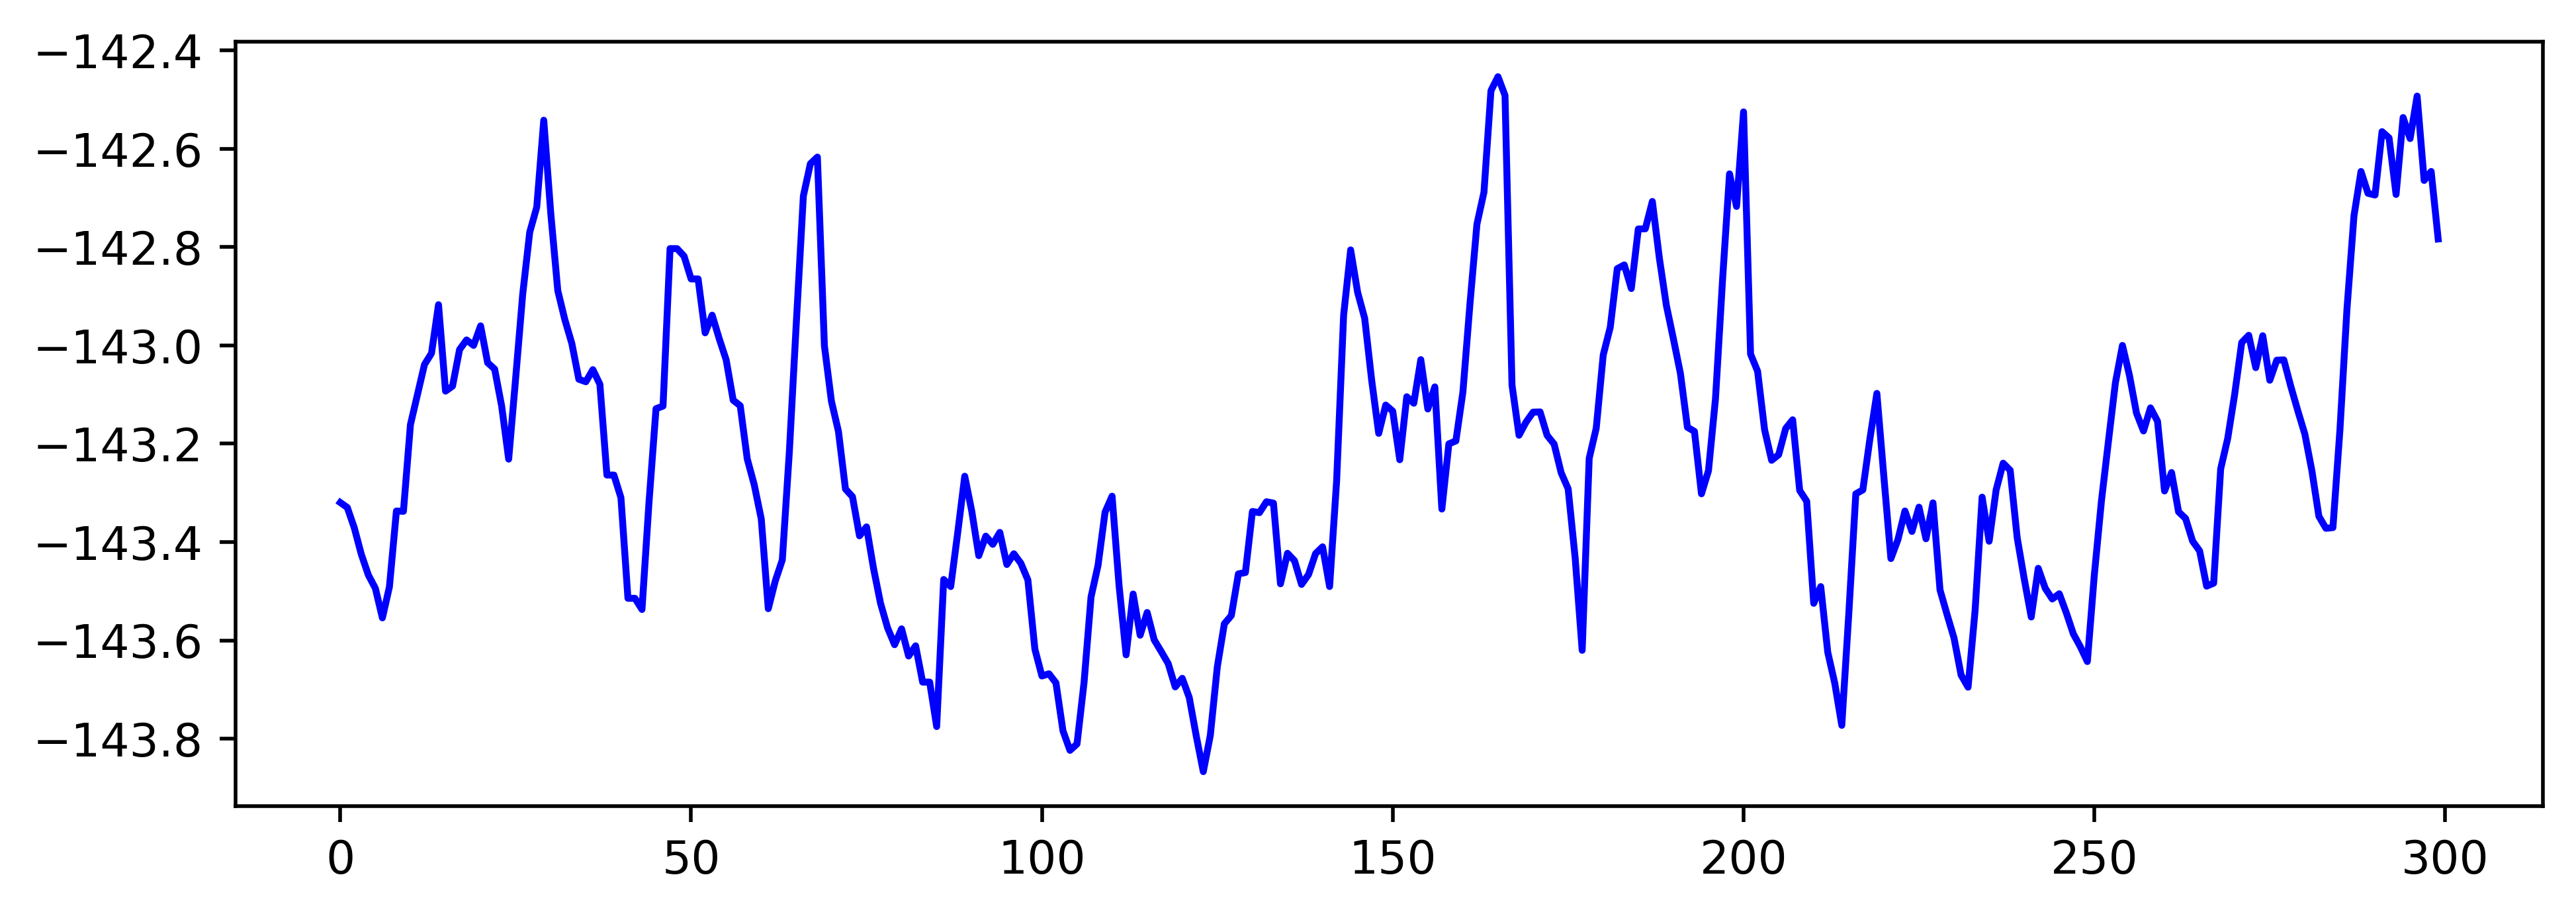
\includegraphics[width=0.45\linewidth]{img/samples/butppg_111001.png} 
			& 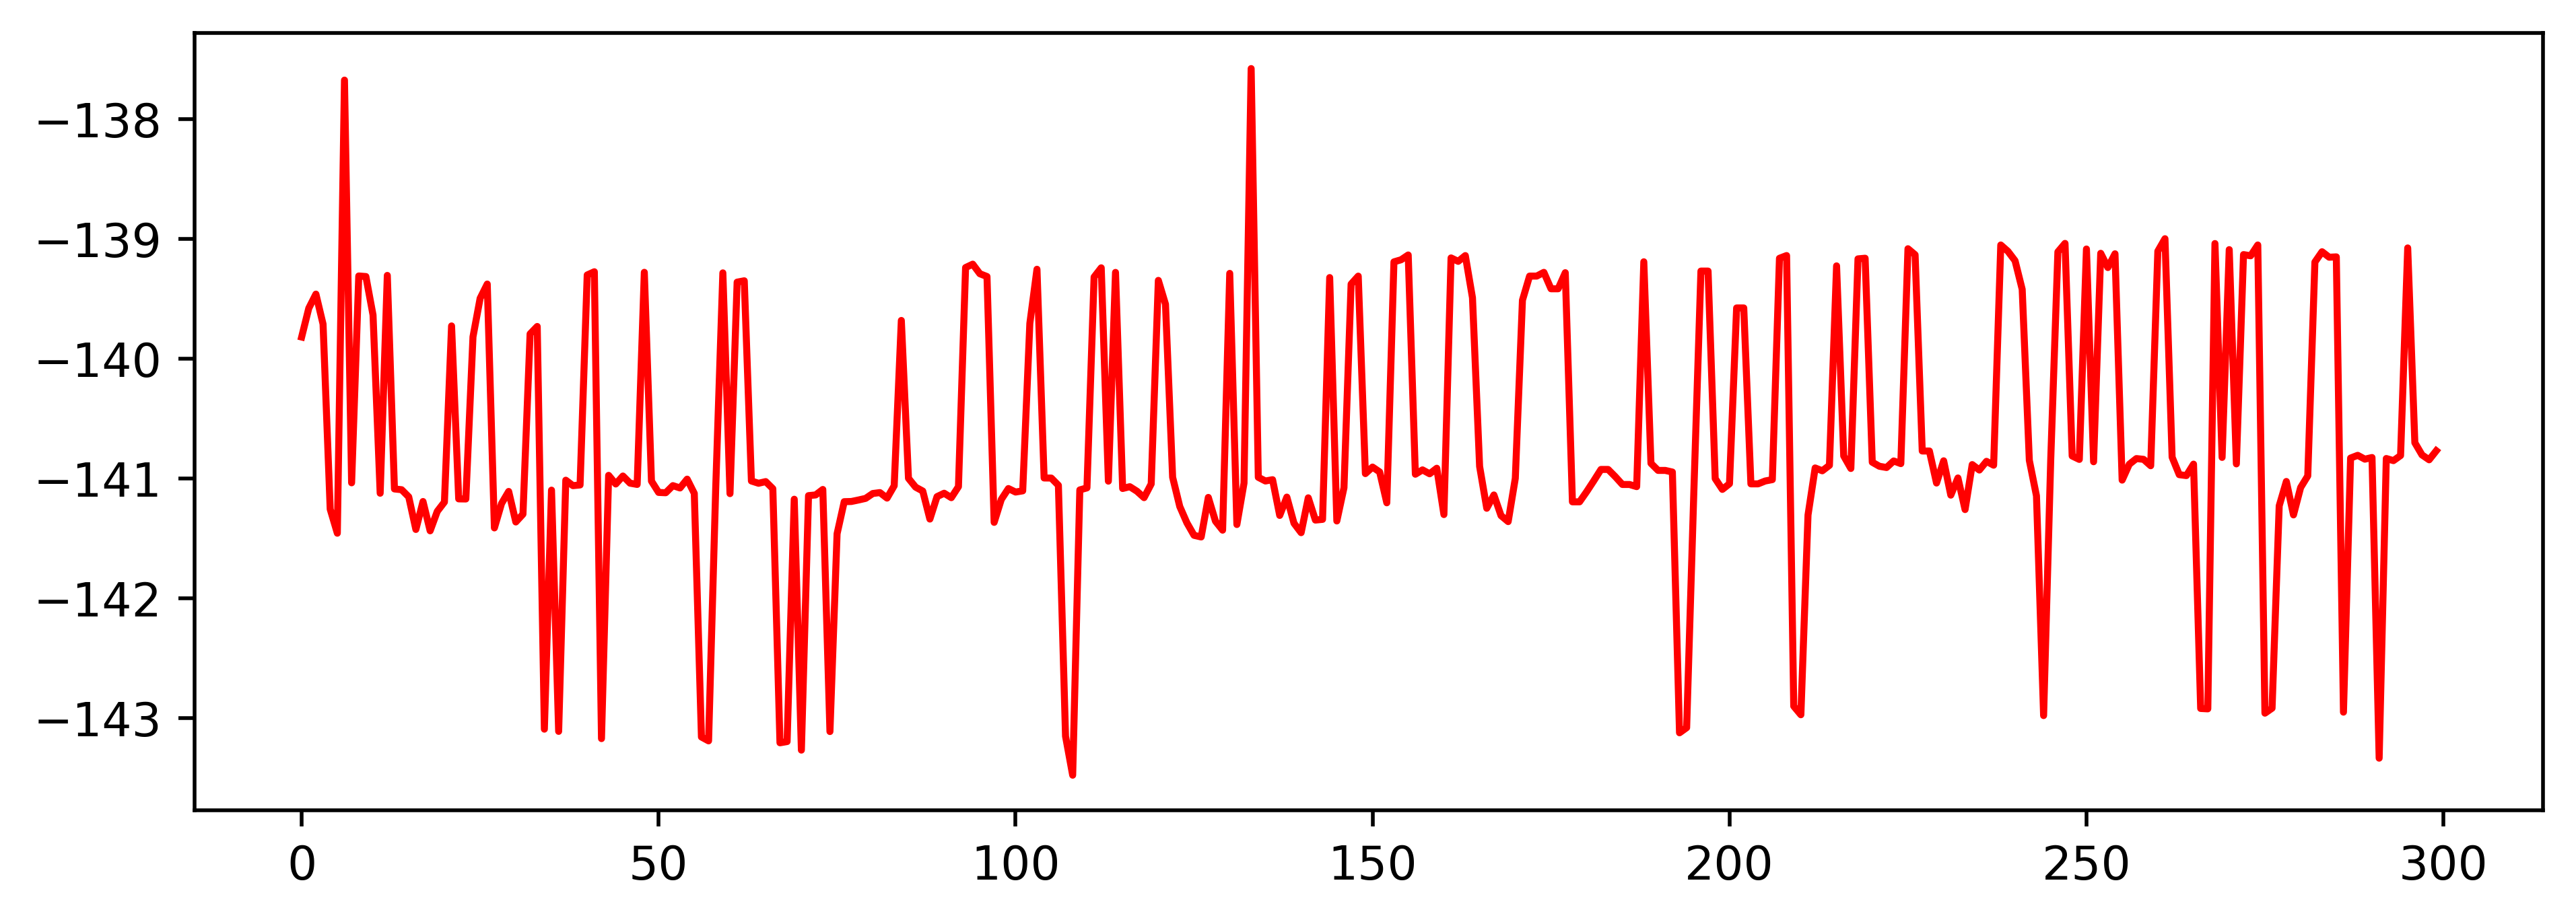
\includegraphics[width=0.45\linewidth]{img/samples/butppg_111003.png} \\
		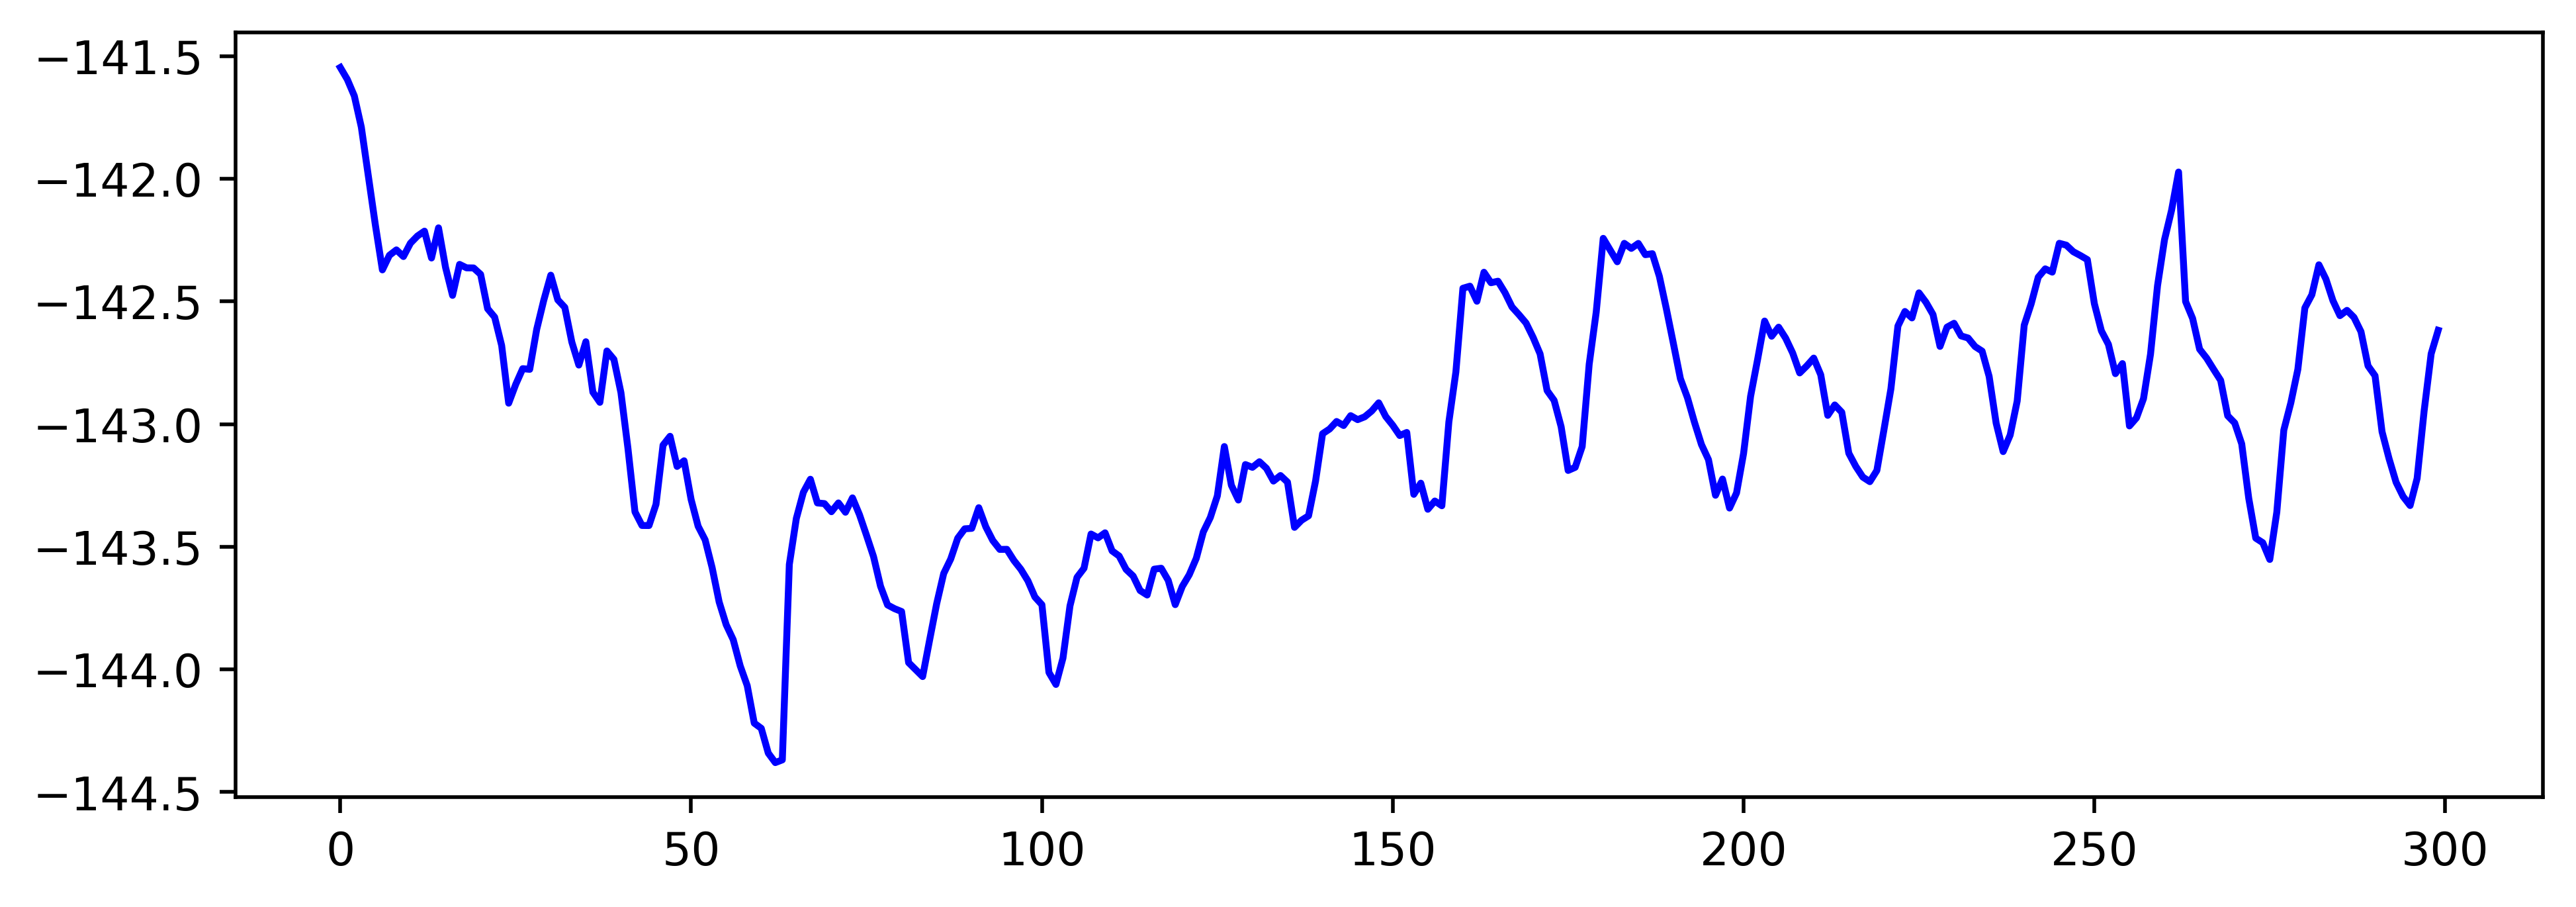
\includegraphics[width=0.45\linewidth]{img/samples/butppg_111002.png} 
			& 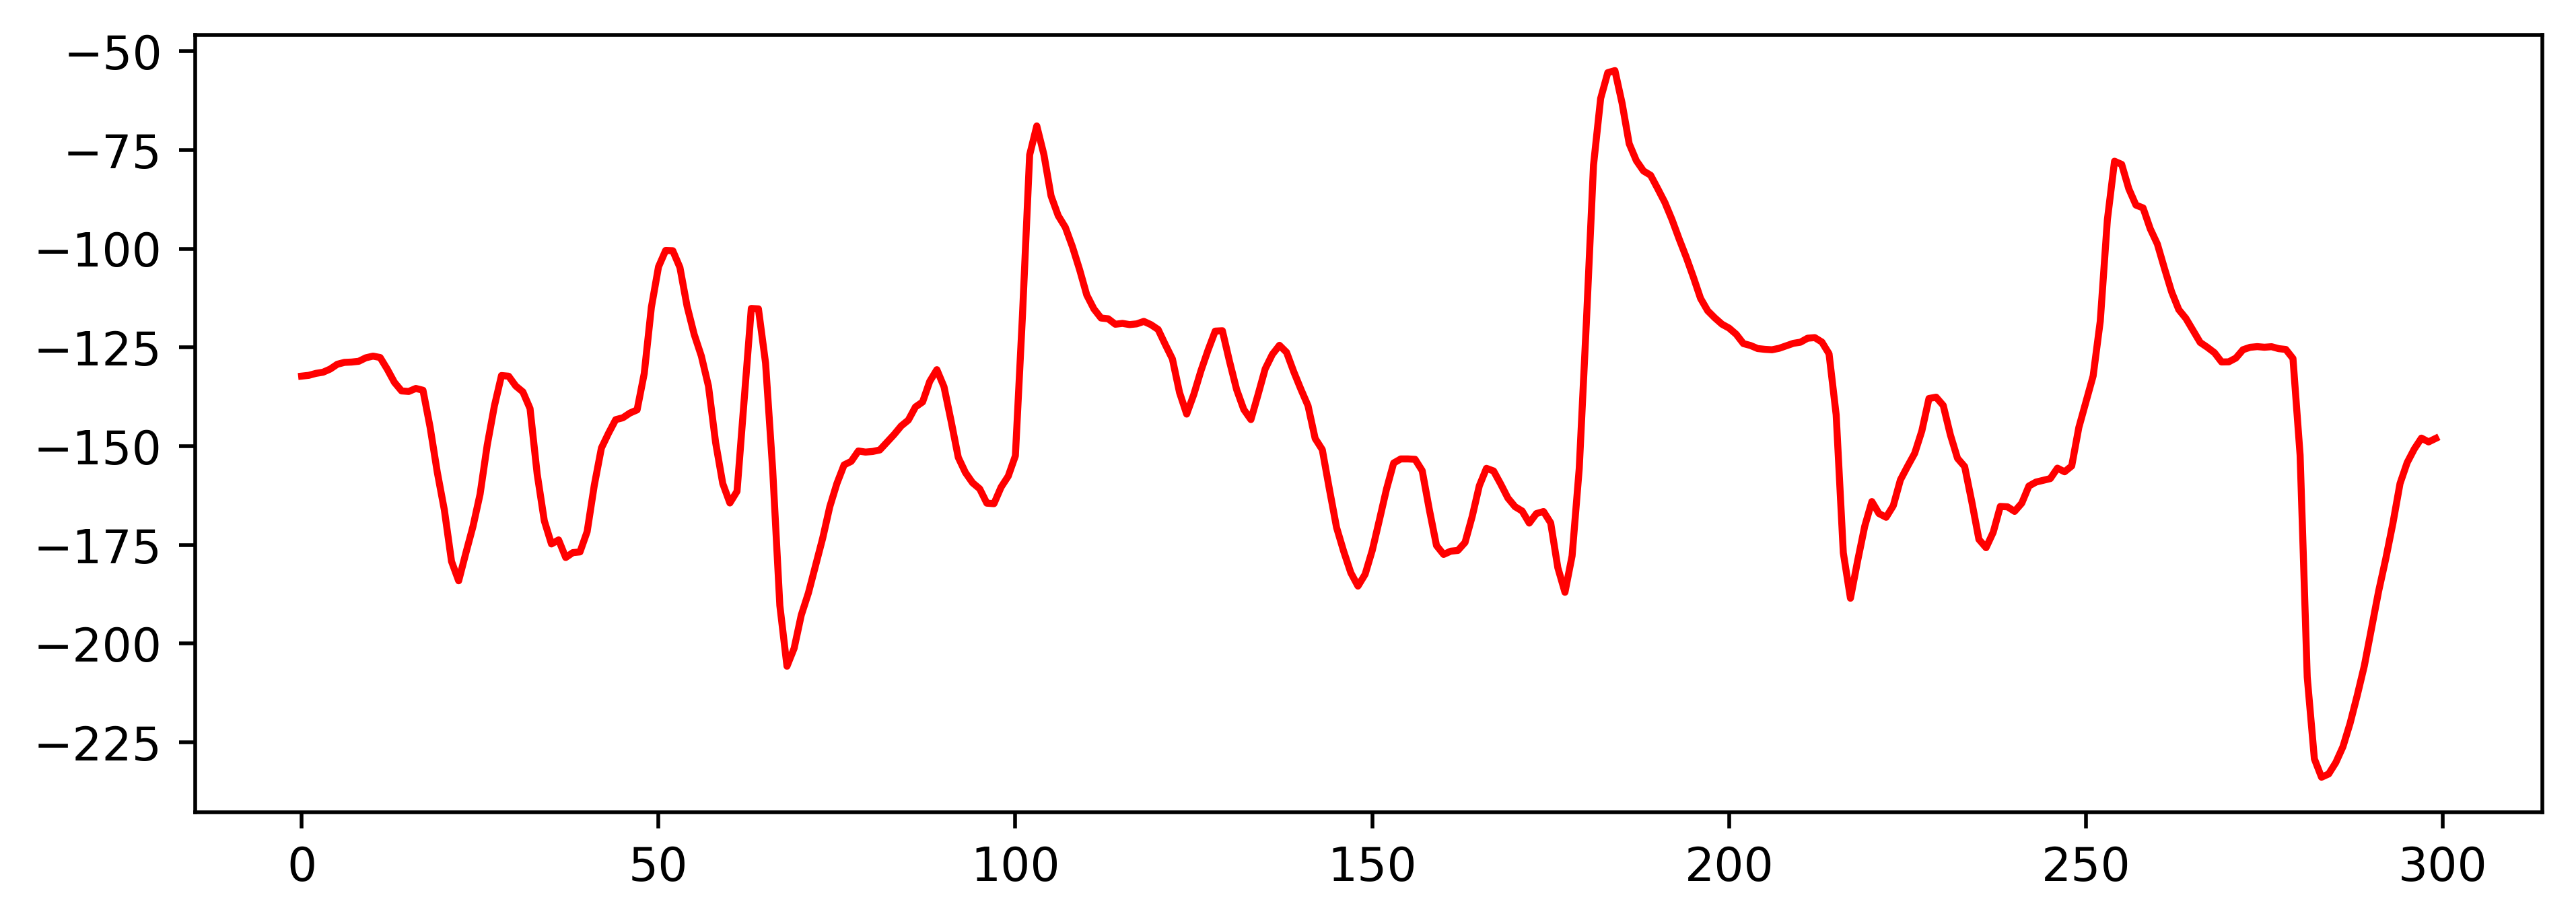
\includegraphics[width=0.45\linewidth]{img/samples/butppg_111004.png} \\
	\end{tabular}
	\caption{Samples of the four signals of the subject with id equal to 11 (where the first subject has id 0). The ``Good'' signals color is blue, while the ``Bad'' signals are red. In those graphs, the vertical dimension is the average of all pixels intensity in a frame, while the horizontal dimension is the time instant in frames. Notice that, since those records are 10 seconds long, it's implied that the sampling frequency is 30 Hz.}
	\label{fig:butppg_samples}
\end{figure}


The \acrfull{BUTPPG} is a publicly available database produced by the Department of Biomedical Engineering of the the Brno University of Technology. It contains samples of \acrshort{PPG} signals, its quality labels and its heat rate estimations. Those signals were extracted using a low-cost method: recording with the camera of a smartphone. To be more precise, they recorded the subject's index finger, covering the lens of the camera and its LED light. Then, they measured, for each video frame, the average of the intensities of the red channel of every image pixel, resulting in a time series of averages. Finally, they inverted the signal. The Figure \ref{fig:butppg_samples} shows examples of the results of such a sequence of procedures.  

They done this method of obtaining \acrshort{PPG} signals  48 times, ammount distributed equally between 12 subjects. That is, for each subject, they did 4 measurements. Moreover, they did those recordings in two possible situations: one which the subject sat down and stayed static, case which the quality label ``Good'' was probable; and other in which the subject walked, hence, case likely to be a ``Bad'' recording. That distinction is relevant, since the walking situation occurred only 1 time for each subject, biasing the labels proportion to be nearly 25\% of ``Bad'' ones. Therefore, this dataset is imbalanced, factor that we need to handle in our experiment.

As for the definition of the signal quality labels, they designated specialists to estimate the heart rate associated with the \acrshort{PPG} signals, with the help of a software specialized for the analysis. Then, the organizers compared the number they gave with the one given by a gold standard method that, instead of using the \acrshort{PPG} signal, used an ECG recording. The measurer syncronized the ECG mannually. If the specialist measured with an error less or equal than 5 bpm, then the organizers considered the estimative correct. Finally, if 3 specialists of 5 gave correct estimations, the organizers considered the quality of the \acrshort{PPG} signal as correct. Thus, the dataset ``Good'' labels, in essence, identify if a signal is human-readable. 

\subsection{The dataset split}

Machine learning tasks also requires the separation the dataset into fragments. One of them is the training dataset, used for the models parameters adjustment. Another is the test dataset, used for evaluating the models efficiency. An optional one is the validation dataset, used to choose the set of best hyperparameters of a trained models. In this experiment case, to define the training-test splits, I used a cross validation method named \acrfull{LOSO}, which partitions the dataset into k pieces and k train-test splits. It makes the i-th train-test split assigning the i-th piece as the test dataset, lefting the other k-1 pieces as the training dataset. In the \acrshort{BUTPPG} case, the k value is 12, the number of subjects. Notice that the smaller unity of division is the subject, not the signals that are associated with it. I did it to increase the difference between training samples and testing samples. Since the dataset is small, such a split method allows the maximum provect of the avaliable resources, because it uses every sample in the dataset as a test object at least once, without biasing the results. Additionally, the training datset was divided producing a validation dataset of size 3, with usage that will be explained later.

\subsection{The models}

To evaluate the proposed projection-based framework, besides comparing it with other existing approaches, which was done using the Aeon toolkit python library, with models listed in table \ref{tab:non_cv_list}, it's necessary to combine it with various classification models which, in that case, are computational vision based. Such a kind of models were implemented in the pytorch python library, in which a wide variety of neural network design strategies were used, as pure convolutional networks, which use the convolution operation to extract features reducing 2d images into smaller ones; residual networks, which uses bypass links between further layers; transformers, that combines the convolution operation with language processing self attention mecanisms; parameter optmized networks, which focuses on having the best parameters selection; models optimized for mobile applications; and more. The table \ref{tab:cv_list} lists all \acrshort{CV} models involved in the experiment.


\begin{table}
	\centering
	\begin{tabular}{llcc}
		\toprule	
		Classification 		& Model 		& Reference 			\\
 		\midrule	
		Transformer    		& Vision Transformer	& \cite{VisionTransformer}	\\
			   		& MaxViT		& \cite{MaxViT}			\\
			   		& Swin Transformer	& \cite{SwinTransformer}	\\
			   		& Swin Transformer V2	& \cite{SwinTransformerV2}	\\
		Residual Net   		& ResNet		& \cite{ResNet}			\\
			 		& ResNeXt		& \cite{ResNeXt}		\\
			 		& WideResNeXt		& \cite{WideResNet}		\\
		Extreme Net	   	& DenseNet		& \cite{DenseNet}		\\
				 	& VGG			& \cite{VGG}			\\
					& SqueezeNet		& \cite{SqueezeNet}		\\
		Mobile Oriented		& MNASNet		& \cite{MNASNet}		\\
					& MobileNet V2		& \cite{MobileNetV2}		\\
					& MobileNet V3		& \cite{MobileNetV3}		\\
		Efficiency Oriented	& EfficientNet		& \cite{EfficientNet}		\\
					& EfficientNet V2	& \cite{EfficientNetV2}		\\
					& ShuffleNet V2		& \cite{ShuffleNetV2}		\\
		Diverse		  	& AlexNet		& \cite{AlexNet}		\\
					& ConvNeXt		& \cite{ConvNeXt}		\\
 					& RegNet		& \cite{RegNet}			\\
		\bottomrule
	\end{tabular}
	\caption{\acrlong{CV} models list, containing its citations.}
	\label{tab:cv_list}
\end{table}



\begin{table}
	\centering
	\adjustbox{width=0.8\textwidth}{
	\begin{tabular}{llc}
		\toprule	
		Classification 		& Model 				& Reference 			\\
 		\midrule	
 		Convolution-Based	& Arsenal				& \cite{HIVECOTEV2}		\\
 					& Rocket Classifier			& \cite{RocketClassifier}	\\
 		Deep Learning		& CNN Classifier			& \cite{CNNClassifier}		\\
 					& FCN Classifier			& \cite{FCNClassifier-MLPClassifier}\\
 					& MLP Classifier			& \cite{FCNClassifier-MLPClassifier}\\
 					& Inception Time Classifier		& \cite{Inception1}\cite{Inception2}\\
 					& Individual Inception Classifier	& \cite{Inception1}\cite{Inception2}\\
 					& LITE Time Classifier			& \cite{LITETimeClassifier}	\\
 		Dictionary-Based	& BOSS Ensemble				& \cite{BOSSEnsemble}		\\
 					& Contractable BOSS			& \cite{ContractableBOSS}	\\
 					& Individual BOSS			& \cite{BOSSEnsemble}		\\
 					& Individual TDE			& \cite{TDE}			\\
 					& MUSE					& \cite{MUSE}			\\
 					& TemporalDictionaryEnsemble		& \cite{TDE}			\\
 					& WEASEL				& \cite{WEASEL}			\\
 					& WEASEL V2				& \cite{WEASELV2}		\\
 					& REDCOMETS				& \cite{REDCOMETS-1}\cite{REDCOMETS-2}\\
 		Distance-Based		& Elastic Ensemble			& \cite{ElasticEnsemble}			\\
 					&					& \cite{}			\\
 					&					& \cite{}			\\
 		Feature-Based		&					& \cite{}			\\
 					&					& \cite{}			\\
 		Hybrid			&					& \cite{}			\\
 					&					& \cite{}			\\
 		Inverval-Based		&					& \cite{}			\\
 					&					& \cite{}			\\
 		Shapelet-Based		&					& \cite{}			\\
 					&					& \cite{}			\\
 		Early Classification	&					& \cite{}			\\
 					&					& \cite{}			\\
 		Ordinal Classification	&					& \cite{}			\\
 					&					& \cite{}			\\
 		Other			&					& \cite{}			\\
 					&					& \cite{}			\\
 		
 		
 		
		\bottomrule
	\end{tabular}
	}
	\caption{Non-\acrlong{CV} models list, containing its citations.}
	\label{tab:non_cv_list}
\end{table}


Even though the models were estabilished, it was still missing the choice of their hyperparameters, that is, high level parameters that doesn't change during the training procedure. For the Aeon models, default hyperparameters were set. But, for the computational vision model, while most of them were set to default, hyperparameter search was done for the learning rate hyperparameter, used in the training. That seach was done applying the Optuna python library, which does heuristic search over the values of the model performance on the validation dataset, in terms of accuracy, to try to find the optimal combination of parameters without testing cases exhaustively. With the finallity of reducing the search space, ramifications the search-space tree can be prunned with a variety of methods, of which median prunning was chosen. Therefore, it was possible to search for the best setting of hyperparameters in a reasonable ammount of time.

\subsection{The training strategy}

Given the before-mentioned models, the dataset and its divisions, it is needed to estabilish a training method for the models parameters adjustment. Since the Aeon implementation already contained a default training procedure, it was only necessary to estabilish the fitting framework for the pytorch computational vision models and the data feeding method. The data feeding was implement using the Data Loader pytorch solution, configuring it to load in batches of size 32. However, before constructing those batches, it was applied a random over sampling, since, as already mentioned, the dataset was unbalanced. As for the pytorch models fitting, the Adam optimizer was used to minimize the Cross Entropy loss function, with and ammount of epochs limited by an early stop technique. In such an early stopping, it is evaluated the median of the absolute deviation values of the last 10 epochs centered in their median. If the obtained number absolute value was less or equal than $0.1$, the training stops. With that estabilished, it is only left to determine the metrics to be measured.     

\subsection{The measurements}

Finally, it's necessary to chose the metrics, used to evaluate objectivelly the solution efficacy. The metrics to be used, in this work, can be separated into two groups: prediction metrics, which measures the quality of the models signal quality assessments; and benchmarking metrics, which measures resources usage and viability. The prediction metrics used were the accuracy, which measure the proportion of correct predictions over all that were made; the precision and the recall, which, similarly to the accuracy, measures the right answers, but for the subsets of all ``Good'' predictions and of all ``Good'' samples, respectively; the f1-score, which combine the precision and the recall into one metric by calculating the harmonice mean between them; and, lastly, the Cohen Kappa score, which measures the simillarity between the observed agreement proportion and the expected agreement probability. Those metrics are summarized in ?. Regarding the benchmarking metrics, it was measured the memory usage in bytes of the model and the inference time (added to the 1d-to-2d projection time for the projection-based models) in seconds.

\begin{equation} \label{eq:Precision}
Precision = \frac{TP}{TP+FP}
\end{equation}


\begin{equation} \label{eq:Recall}
Recall = \frac{TP}{TP+FN}
\end{equation}

\begin{equation} \label{eq:F1-Score}
\Mathenize{F1-Score}  = \Mathenize{Harmonic-Mean}(Precision,Recall) 
\end{equation}


\begin{equation} 
p_o = \frac{TP+TN}{TP+TN+FP+FN}
\end{equation}

\begin{equation}
p_e  = \mathbb{P}(f(X)=p) \cdot \mathbb{P}(y=p) + \mathbb{P}(f(X)=n) \cdot \mathbb{P}(y=n)
\end{equation}

\begin{equation} \label{eq:Cohen Kappa}
Cohen Kappa  = \frac{p_o - p_e}{1 - p_e} 
\end{equation}

\subsection{The overall schema}

Reviewing what was presented, the experiment will begin by splitting the \acrshort{BUTPPG} dataset using simple division for the purpose of, subsequentially, selecting the best hyperparameters of the \acrshort{CV} models. With the best hyperparameters chosen, all models, including the non \acrshort{CV} models, will be evaluated using the \acrshort{LOSO} strategy, producing the metrics for each fold.


\section{Experimental results}


In this section, the results will be analyzed by comparing the metrics in the following order: firstly, the Cohen Kappa Score, verifying if it's value is superior o equal to 90\%; then, the F1-Score; and, finally, the Precision score. Moreover, it will be considered the trade-off between models with respect to the inference time and the memory consumption. Since a large set of models was considered, the model comparision was done in sections, accordingly to the before-presented computer vision model classifications: Transformers, Residual nets, Parameter efficiency, Mobile nets and Diverse. In each of those sections, the best combinatons of model variant and projection method will be selected, if at least one of them is sufficiently good. Afterwards, the selections of each section will be compared, also discussing the differences between the projection methods. Lastly, the best combinations of models variants and projection methods will be compared to the best standard time series classification models present in the Aeon toolkit.

\pagebreak

\subsection{Categories analysis}

\subsubsection{Transformers}

Three transformers were considered: the Vision Transformer, the Multi-axis Vision Transformer and the Shifted Windows Transformer. Firsly, observing the tables \ref{tab:Averages_of_VisionTransformer} \ref{tab:Averages_of_SwinTransformer} \ref{tab:Averages_of_Maxvit}, it's noticeable that only some variants of the Vision Transformer obtained Cohen Kappa scores superior than 90\%, while the tiny Swin Transformer obtained almost 90\% in the same score. The highest Cohen Kappa scores and F1-scores were obtained by the large Vision Transformer variants for the \acrshort{RP} and \acrshort{Mix} projection methods, in contrast to the huge variant, that performed significantly worse for all projections. Specifically, the models Vision Transformer L 16, with \acrshort{RP} and \acrshort{Mix} and Vision Transformer L 32 with \acrshort{Mix} obtained the best scores, while having similar memory consumption and a sighly difference in inference time, with the 32x32 patch sized variant being the slowest, fact observed in the figure \ref{fig:Time_of_Transformers}. One drawback of the Vision Transformer models, if compared to the other transformers in this section, is that its memory consumption is drastically higher, as exposed in the table \ref{tab:Memory_of_Transformers}. Regardless, the Vision Transformer L 16 with \acrshort{RP} was selected as the best model of this section, since this model was, primally, one of those that achieved the highest score, and, if compared with the Vision Transformer L 32 and with the \acrshort{Mix} projection, was the fastest in inference speed.

\pagebreak

\AveragesTable{Vision Transformer}{VisionTransformer}
\AveragesTable{MaxViT}{Maxvit}
\AveragesTable{Swin Transformer~V2}{SwinTransformer}
\AveragesTable{Swin Transformer~V2}{SwinTransformerV2}


\IncludeMemoryTable{Transformers}

\begin{figure}[h!]
	\includegraphics[width=\timePlotsWidth]{img/resultados/boxplots/benchmark_of_VisionTransformer.pdf}
	\includegraphics[width=\timePlotsWidth]{img/resultados/boxplots/benchmark_of_SwinTransformer.pdf}
	\includegraphics[width=\timePlotsWidth]{img/resultados/boxplots/benchmark_of_SwinTransformer V2.pdf}
	\includegraphics[width=\timePlotsWidth]{img/resultados/boxplots/benchmark_of_MaxVit.pdf}
	\caption{\TimePlotsDescription{Transformers}}
	\label{fig:Time_of_Transformers}
\end{figure}


\pagebreak

\subsubsection{ResNet based}

This section contains the ResNet itself and two derivated models, the Wide ResNet, a model with more channels per block; and the ResNeXt, a model that, as oposed to the before-mentioned wide in channels model, employs an multipath philosophy, agreggating the paths by an additive operation. As it's clear in the table \ref{tab:Averages_of_ResNeXt}, every ResNeXt variant didn't obtained a sufficient Cohen Kappa score, which was the case for the Wide Res Net with 101 layers and 2 convolutions per block combined with the \acrshort{Mix} projection, as seen in \ref{tab:Averages_of_WideResNet}; and for the ResNets variants with 50 and 101 layers and the \acrshort{Mix} projection as well,  as seen in \ref{tab:Averages_of_ResNet}. Comparing these last variants, it can be concluded that the Wide ResNet 101-2 variant with the \acrshort{Mix} method obtained the best score, both for Cohen Kappa and F1 scores. However, that Wide ResNet posesses the largest memory occupation, according to the table \ref{tab:Memory_of_ResNet based}, and spends the fourth higher inference time, as seen in the figure \ref{fig:Time_of_ResNet based}.  Despite this disavantage, the Wide ResNet 101-2 variant with the \acrshort{Mix} was the choice of this section.

\pagebreak


\AveragesTable{ResNet}{ResNet}
\AveragesTable{ResNeXt}{ResNeXt}
\AveragesTable{Wide ResNet}{WideResNet}



\IncludeMemoryTable{ResNet based}

\begin{figure}[h!]
	\includegraphics[width=\timePlotsWidth]{img/resultados/boxplots/benchmark_of_ResNet.pdf}
	\includegraphics[width=\timePlotsWidth]{img/resultados/boxplots/benchmark_of_Wide ResNet.pdf}
	\includegraphics[width=\timePlotsWidth]{img/resultados/boxplots/benchmark_of_ResNeXt.pdf}
	\caption{\TimePlotsDescription{Residual Nets}}
	\label{fig:Time_of_ResNet based}
\end{figure}


\FloatBarrier

\subsubsection{Purely Convolutional}

In this section, the AlexNet, a classic model, and the ConvNeXt, a mordenized pure convolutional network, are present. As seen in tables \ref{tab:Averages_of_AlexNet} and \ref{tab:Averages_of_ConvNeXt}, only the AlexNet combined with the \acrshort{Mix} projection method obtained a CohenKappa score superior than 90\%, while achieving a very fast inference speed, with less than 20 ms latency, and comparable to the ConvNeXt memory occupation. Therefore, such combination was selected.  

\begin{table}[h!]
	\adjustbox{width=\averagesTableWidth,center}{
		
\begin{tabular}{lllll}
\toprule
Model & Projection & Cohen Kappa & F1 Score & Precision \\
\midrule
ConvNeXt: Base & GAF & \textcolor[rgb]{0.8501939719,0.1498060281,0}{0.536} $\pm$ \textcolor[rgb]{0.4498340830,0.5000000000,0}{0.157} & \textcolor[rgb]{0.9819518717,0.0180481283,0}{0.792} $\pm$ \textcolor[rgb]{0.6916472560,0.3083527440,0}{0.137} & \textcolor[rgb]{0.6500000000,0.3500000000,0}{0.764} $\pm$ \textcolor[rgb]{0.2890812278,0.5000000000,0}{0.170} \\
 & MTF & \textcolor[rgb]{1.0000000000,0.0000000000,0}{0.473} $\pm$ \textcolor[rgb]{0.3758318907,0.5000000000,0}{0.144} & \textcolor[rgb]{1.0000000000,0.0000000000,0}{0.789} $\pm$ \textcolor[rgb]{1.0000000000,0.0000000000,0}{0.159} & \textcolor[rgb]{1.0000000000,0.0000000000,0}{0.667} $\pm$ \textcolor[rgb]{1.0000000000,0.0000000000,0}{0.268} \\
 & RP & \textcolor[rgb]{0.0295434199,0.5000000000,0}{0.883} $\pm$ \textcolor[rgb]{0.5955244630,0.4044755370,0}{0.184} & \underline{\textcolor[rgb]{0.2319518717,0.5000000000,0}{0.913}} $\pm$ \textcolor[rgb]{0.9235235198,0.0764764802,0}{0.154} & \underline{\textbf{\textcolor[rgb]{0.0000000000,0.5000000000,0}{0.944}}} $\pm$ \textbf{\textcolor[rgb]{0.0000000000,0.5000000000,0}{0.130}} \\
 & Mix & \textcolor[rgb]{0.0984780662,0.5000000000,0}{0.854} $\pm$ \textcolor[rgb]{0.6747481909,0.3252518091,0}{0.198} & \underline{\textcolor[rgb]{0.1510695187,0.5000000000,0}{0.926}} $\pm$ \textcolor[rgb]{0.0999682822,0.5000000000,0}{0.093} & \underline{\textcolor[rgb]{0.0750000000,0.5000000000,0}{0.924}} $\pm$ \textcolor[rgb]{0.0718829596,0.5000000000,0}{0.140} \\
ConvNeXt: Large & GAF & \textcolor[rgb]{0.6729334527,0.3270665473,0}{0.611} $\pm$ \textcolor[rgb]{0.8999515496,0.1000484504,0}{0.239} & \textcolor[rgb]{0.6510695187,0.3489304813,0}{0.845} $\pm$ \textcolor[rgb]{0.5159088943,0.4840911057,0}{0.124} & \textcolor[rgb]{0.5750000000,0.4250000000,0}{0.785} $\pm$ \textcolor[rgb]{0.3827984820,0.5000000000,0}{0.183} \\
 & MTF & \textcolor[rgb]{0.8281110116,0.1718889884,0}{0.545} $\pm$ \textcolor[rgb]{0.4139672114,0.5000000000,0}{0.151} & \textcolor[rgb]{0.6265597148,0.3734402852,0}{0.849} $\pm$ \textcolor[rgb]{0.2093230731,0.5000000000,0}{0.101} & \textcolor[rgb]{0.7000000000,0.3000000000,0}{0.750} $\pm$ \textcolor[rgb]{0.1516428390,0.5000000000,0}{0.151} \\
 & RP & \textcolor[rgb]{0.0787824530,0.5000000000,0}{0.862} $\pm$ \textcolor[rgb]{0.5941088240,0.4058911760,0}{0.184} & \textcolor[rgb]{0.3348930481,0.5000000000,0}{0.896} $\pm$ \textcolor[rgb]{0.9311751943,0.0688248057,0}{0.154} & \underline{\textbf{\textcolor[rgb]{0.0000000000,0.5000000000,0}{0.944}}} $\pm$ \textbf{\textcolor[rgb]{0.0000000000,0.5000000000,0}{0.130}} \\
 & Mix & \textcolor[rgb]{0.0787824530,0.5000000000,0}{0.862} $\pm$ \textcolor[rgb]{0.5941088240,0.4058911760,0}{0.184} & \textcolor[rgb]{0.3348930481,0.5000000000,0}{0.896} $\pm$ \textcolor[rgb]{0.9311751943,0.0688248057,0}{0.154} & \underline{\textbf{\textcolor[rgb]{0.0000000000,0.5000000000,0}{0.944}}} $\pm$ \textbf{\textcolor[rgb]{0.0000000000,0.5000000000,0}{0.130}} \\
ConvNeXt: Small & GAF & \textcolor[rgb]{0.4431512981,0.5000000000,0}{0.708} $\pm$ \textcolor[rgb]{1.0000000000,0.0000000000,0}{0.257} & \textcolor[rgb]{0.4059714795,0.5000000000,0}{0.885} $\pm$ \textcolor[rgb]{0.5007263060,0.4992736940,0}{0.123} & \textcolor[rgb]{0.4000000000,0.5000000000,0}{0.833} $\pm$ \textcolor[rgb]{0.4683369943,0.5000000000,0}{0.195} \\
 & MTF & \textcolor[rgb]{0.6729334527,0.3270665473,0}{0.611} $\pm$ \textcolor[rgb]{0.8999515496,0.1000484504,0}{0.239} & \textcolor[rgb]{0.6510695187,0.3489304813,0}{0.845} $\pm$ \textcolor[rgb]{0.5159088943,0.4840911057,0}{0.124} & \textcolor[rgb]{0.5750000000,0.4250000000,0}{0.785} $\pm$ \textcolor[rgb]{0.3827984820,0.5000000000,0}{0.183} \\
 & RP & \textcolor[rgb]{0.0984780662,0.5000000000,0}{0.854} $\pm$ \textcolor[rgb]{0.6747481909,0.3252518091,0}{0.198} & \underline{\textcolor[rgb]{0.1510695187,0.5000000000,0}{0.926}} $\pm$ \textcolor[rgb]{0.0999682822,0.5000000000,0}{0.093} & \underline{\textcolor[rgb]{0.0750000000,0.5000000000,0}{0.924}} $\pm$ \textcolor[rgb]{0.0718829596,0.5000000000,0}{0.140} \\
 & Mix & \textbf{\textcolor[rgb]{0.0000000000,0.5000000000,0}{0.896}} $\pm$ \textcolor[rgb]{0.5039453787,0.4960546213,0}{0.167} & \underline{\textcolor[rgb]{0.0775401070,0.5000000000,0}{0.938}} $\pm$ \textcolor[rgb]{0.0931749808,0.5000000000,0}{0.093} & \underline{\textbf{\textcolor[rgb]{0.0000000000,0.5000000000,0}{0.944}}} $\pm$ \textbf{\textcolor[rgb]{0.0000000000,0.5000000000,0}{0.130}} \\
ConvNeXt: Tiny & GAF & \textcolor[rgb]{0.4923903312,0.5000000000,0}{0.688} $\pm$ \textcolor[rgb]{0.9113745311,0.0886254689,0}{0.241} & \textcolor[rgb]{0.4108734403,0.5000000000,0}{0.884} $\pm$ \textcolor[rgb]{0.2082138349,0.5000000000,0}{0.101} & \textcolor[rgb]{0.4250000000,0.5000000000,0}{0.826} $\pm$ \textcolor[rgb]{0.2789740494,0.5000000000,0}{0.168} \\
 & MTF & \textcolor[rgb]{0.8818263205,0.1181736795,0}{0.523} $\pm$ \textbf{\textcolor[rgb]{0.0000000000,0.5000000000,0}{0.075}} & \textcolor[rgb]{0.7295008913,0.2704991087,0}{0.833} $\pm$ \textcolor[rgb]{0.0562553209,0.5000000000,0}{0.090} & \textcolor[rgb]{0.7000000000,0.3000000000,0}{0.750} $\pm$ \textcolor[rgb]{0.1516428390,0.5000000000,0}{0.151} \\
 & RP & \textcolor[rgb]{0.2790211877,0.5000000000,0}{0.778} $\pm$ \textcolor[rgb]{0.9977538235,0.0022461765,0}{0.257} & \underline{\textcolor[rgb]{0.2932263815,0.5000000000,0}{0.903}} $\pm$ \textcolor[rgb]{0.3666523082,0.5000000000,0}{0.113} & \textcolor[rgb]{0.2500000000,0.5000000000,0}{0.875} $\pm$ \textcolor[rgb]{0.1960820797,0.5000000000,0}{0.157} \\
 & Mix & \textcolor[rgb]{0.0492390331,0.5000000000,0}{0.875} $\pm$ \textcolor[rgb]{0.6812870810,0.3187129190,0}{0.199} & \underline{\textbf{\textcolor[rgb]{0.0000000000,0.5000000000,0}{0.951}}} $\pm$ \textbf{\textcolor[rgb]{0.0000000000,0.5000000000,0}{0.086}} & \underline{\textcolor[rgb]{0.0181818182,0.5000000000,0}{0.939}} $\pm$ \textcolor[rgb]{0.0367461744,0.5000000000,0}{0.135} \\
\bottomrule
\end{tabular}


	}
	\caption{\AveragesTableDescription{ConvNeXt}}
	\label{tab:Averages_of_ConvNeXt}
\end{table}

\begin{table}[h!]
	\adjustbox{width=\averagesTableWidth,center}{
		
\begin{tabular}{lllll}
\toprule
Model & Projection & Cohen Kappa & F1 Score & Precision \\
\midrule
AlexNet & GAF & \textcolor[rgb]{1.0000000000,0.0000000000,0}{0.545} $\pm$ \textbf{\textcolor[rgb]{0.0000000000,0.5000000000,0}{0.151}} & \textcolor[rgb]{0.7777777778,0.2222222222,0}{0.849} $\pm$ \textcolor[rgb]{0.1993959038,0.5000000000,0}{0.101} & \textcolor[rgb]{1.0000000000,0.0000000000,0}{0.750} $\pm$ \textcolor[rgb]{0.6349071673,0.3650928327,0}{0.151} \\
 & MTF & \textcolor[rgb]{0.8571428571,0.1428571429,0}{0.598} $\pm$ \textcolor[rgb]{1.0000000000,0.0000000000,0}{0.247} & \textcolor[rgb]{0.9425837321,0.0574162679,0}{0.827} $\pm$ \textcolor[rgb]{1.0000000000,0.0000000000,0}{0.174} & \textcolor[rgb]{0.8831168831,0.1168831169,0}{0.773} $\pm$ \textcolor[rgb]{1.0000000000,0.0000000000,0}{0.163} \\
 & RP & \textcolor[rgb]{0.5724489796,0.4275510204,0}{0.704} $\pm$ \textcolor[rgb]{0.5538521086,0.4461478914,0}{0.204} & \textcolor[rgb]{1.0000000000,0.0000000000,0}{0.819} $\pm$ \textcolor[rgb]{0.9283513413,0.0716486587,0}{0.168} & \underline{\textcolor[rgb]{0.1785714286,0.5000000000,0}{0.910}} $\pm$ \textcolor[rgb]{0.1620976255,0.5000000000,0}{0.135} \\
 & Mix & \underline{\textbf{\textcolor[rgb]{0.0000000000,0.5000000000,0}{0.917}}} $\pm$ \textcolor[rgb]{0.1259027269,0.5000000000,0}{0.163} & \underline{\textbf{\textcolor[rgb]{0.0000000000,0.5000000000,0}{0.955}}} $\pm$ \textbf{\textcolor[rgb]{0.0000000000,0.5000000000,0}{0.083}} & \underline{\textbf{\textcolor[rgb]{0.0000000000,0.5000000000,0}{0.944}}} $\pm$ \textbf{\textcolor[rgb]{0.0000000000,0.5000000000,0}{0.130}} \\
\bottomrule
\end{tabular}


	}
	\caption{\AveragesTableDescription{AlexNet}}
	\label{tab:Averages_of_AlexNet}
\end{table}


\begin{figure}[h!]
	\includegraphics[width=\timePlotsWidth]{img/resultados/boxplots/benchmark_of_AlexNet.pdf}
	\includegraphics[width=\timePlotsWidth]{img/resultados/boxplots/benchmark_of_ConvNeXt.pdf}
	\caption{\TimePlotsDescription{Purely Convolutional}}
	\label{fig:Time_of_Purely Convolutional}
\end{figure}


\IncludeMemoryTable{Purely convolutional}

\FloatBarrier

\subsubsection{Mobile Oriented}

This section contain the mobile oriented networks MNASNet, a mobile plataform aware seach algorithm; Mobile Net V2, which uses inverted residuals and linear bottlenecks to better fit the mobile context; and Mobile Net V3, which combines architectural search with various network improvements. Of those models, only the MNASNet obtained a sufficient Cohen Kappa score, as visible in the tables \ref{tab:Averages_of_MNASNet}, \ref{tab:Averages_of_MobileNet V2} e \ref{tab:Averages_of_MobileNet V3}. Specifically, the MNASNet with depth multiplier of 1.0, that is, with exaclty the same number of channels in each layer of the base model; combined with the \acrshort{Mix} projection method method. According to the table \ref{tab:Memory_of_Mobile nets} and the figure \ref{fig:Time_of_Mobile nets}, all of those networks have very small memory size, with values inferior to 30 MB; and very fast inference time, with medians bellow to 20 ms. For this reason, the MNASNet 1.0 with \acrshort{Mix} was chosen. 

\AveragesTable{MNASNet}{MNASNet}
\AveragesTable{MobileNet~V2}{MobileNetV2}
\AveragesTable{MobileNet~V3}{MobileNetV3}


\IncludeMemoryTable{Mobile nets}

\begin{figure}[h!]
	\includegraphics[width=\timePlotsWidth]{img/resultados/boxplots/benchmark_of_MobileNet V2.pdf}
	\includegraphics[width=\timePlotsWidth]{img/resultados/boxplots/benchmark_of_MobileNet V3.pdf}
	\includegraphics[width=\timePlotsWidth]{img/resultados/boxplots/benchmark_of_MNASNet.pdf}
	\caption{\TimePlotsDescription{Mobile Oriented}}
	\label{fig:Time_of_Mobile nets}
\end{figure}


\FloatBarrier

\subsubsection{RegNet}

In this section, the set of variants of the RegNet networks are analyzed. RegNets are networks selected from a population of networks in a design space, that is, a space of networks resulting from a limited set of hyperparameters. By looking at the table \ref{tab:Averages_of_RegNet}, it can be seen that, of those variants, only 4 got a sufficient Cohen Kappa score: from the RegNet X design space, the 800 MF and 3.2 GF variants; and from the RegNet Y design space, the 400 MF and 800 MF variants. All of those variants obtained such a score by applying the \acrshort{Mix} method, except for the Reg Net Y 400 MF variant, that was combined with the \acrshort{RP} approach. Since all of those variants obtained a similar score in all metrics, the memory usage was considered to select the RegNet Y 400 MF variant, since this model is the smallest in memory occupation, using, according to the table \ref{tab:Memory_of_RegNet}, only 15 MB; even though the RegNet Y variants have, in general, a slower inference speed if compared to the RegNet X counterparts, as sighly noticeable in the figure \ref{fig:Time_of_RegNet}.

\AveragesTable{RegNet}



\IncludeMemoryTable{RegNet}

\begin{figure}[h!]
	\includegraphics[width=\timePlotsWidth]{img/resultados/boxplots/benchmark_of_RegNet.pdf}
	\caption{\TimePlotsDescription{RegNet}}
	\label{fig:Time_of_RegNet}
\end{figure}


\FloatBarrier

\subsubsection{Extreme Nets}

In this section, it's discussed the results of neural models which are an exageration of a concept, as the VGG, which is a model that, for its biggest variants, is a very deep model when considering its number of layers; and the DenseNet, which apply the skipping connections of the residual nets to all pairs of blocks in the network. Accordingly to the tables \ref{tab:Averages_of_DenseNet} and \ref{tab:Averages_of_VGG}, only one variant have succeded to barely achieve an over the quota Cohen Kappa score: the VGG with 16 blocks without Batch Normalization, when combined with the \acrshort{RP} method. Additionally, as presented in the figure \ref{fig:Time_of_Extreme nets}, the VGGs have a considerable lower inference speed, with medians that have values near 20 ms. In contrast, the VGGs are not small-in-memory models, with occupation suprassing 500 MB, as seen in table \ref{tab:Memory_of_Extreme nets}, while the biggest DenseNet occupies 105 MB. Nonetheless, the VGG 16 variant combined with the \acrshort{RP} projection method is selected as the representative model of this section.

\begin{table}[h!]
	\adjustbox{width=\averagesTableWidth,center}{
		
\begin{tabular}[t]{lllll}
\toprule
Model & Projection & Cohen Kappa & F1 Score & Precision \\
\midrule
VGG: 11 & GAF & \textcolor[rgb]{0.5761353517,0.4238646483,0}{0.659} $\pm$ \textcolor[rgb]{0.9813763962,0.0186236038,0}{0.257} & \textcolor[rgb]{0.6130820399,0.3869179601,0}{0.840} $\pm$ \textcolor[rgb]{0.8179931192,0.1820068808,0}{0.182} & \textcolor[rgb]{0.5967365967,0.4032634033,0}{0.811} $\pm$ \textcolor[rgb]{0.6502693890,0.3497306110,0}{0.201} \\
 & MTF & \textcolor[rgb]{0.9501335708,0.0498664292,0}{0.500} $\pm$ \textcolor[rgb]{0.6654355176,0.3345644824,0}{0.174} & \textcolor[rgb]{0.8699186992,0.1300813008,0}{0.790} $\pm$ \textcolor[rgb]{0.4021860668,0.5000000000,0}{0.116} & \textcolor[rgb]{0.8974358974,0.1025641026,0}{0.729} $\pm$ \textcolor[rgb]{0.3672049968,0.5000000000,0}{0.155} \\
 & RP & \textcolor[rgb]{0.1763134461,0.5000000000,0}{0.829} $\pm$ \textcolor[rgb]{0.7355621391,0.2644378609,0}{0.192} & \textcolor[rgb]{0.5365853659,0.4634146341,0}{0.855} $\pm$ \textcolor[rgb]{0.8554220067,0.1445779933,0}{0.188} & \underline{\textcolor[rgb]{0.1025641026,0.5000000000,0}{0.944}} $\pm$ \textcolor[rgb]{0.2080512860,0.5000000000,0}{0.130} \\
 & Mix & \textcolor[rgb]{0.1665182547,0.5000000000,0}{0.833} $\pm$ \textcolor[rgb]{0.8482671723,0.1517328277,0}{0.222} & \underline{\textcolor[rgb]{0.1463414634,0.5000000000,0}{0.931}} $\pm$ \textcolor[rgb]{0.2240040057,0.5000000000,0}{0.087} & \underline{\textcolor[rgb]{0.2564102564,0.5000000000,0}{0.903}} $\pm$ \textcolor[rgb]{0.3075839781,0.5000000000,0}{0.146} \\
VGG: 11 BN & GAF & \textcolor[rgb]{0.8032056990,0.1967943010,0}{0.562} $\pm$ \textcolor[rgb]{0.5940200153,0.4059799847,0}{0.155} & \textcolor[rgb]{0.5691056911,0.4308943089,0}{0.848} $\pm$ \textcolor[rgb]{0.1349899397,0.5000000000,0}{0.073} & \textcolor[rgb]{0.7692307692,0.2307692308,0}{0.764} $\pm$ \textcolor[rgb]{0.2230100982,0.5000000000,0}{0.132} \\
 & MTF & \textcolor[rgb]{0.8432769368,0.1567230632,0}{0.545} $\pm$ \textcolor[rgb]{0.5762840628,0.4237159372,0}{0.151} & \textcolor[rgb]{0.5650406504,0.4349593496,0}{0.849} $\pm$ \textcolor[rgb]{0.3108773772,0.5000000000,0}{0.101} & \textcolor[rgb]{0.8205128205,0.1794871795,0}{0.750} $\pm$ \textcolor[rgb]{0.3384113914,0.5000000000,0}{0.151} \\
 & RP & \textcolor[rgb]{0.0685663402,0.5000000000,0}{0.875} $\pm$ \textcolor[rgb]{0.6443051694,0.3556948306,0}{0.169} & \underline{\textcolor[rgb]{0.1951219512,0.5000000000,0}{0.921}} $\pm$ \textcolor[rgb]{0.2928051170,0.5000000000,0}{0.098} & \underline{\textcolor[rgb]{0.1025641026,0.5000000000,0}{0.944}} $\pm$ \textcolor[rgb]{0.2080512860,0.5000000000,0}{0.130} \\
 & Mix & \textcolor[rgb]{0.1175422974,0.5000000000,0}{0.854} $\pm$ \textcolor[rgb]{0.7578007605,0.2421992395,0}{0.198} & \underline{\textcolor[rgb]{0.1707317073,0.5000000000,0}{0.926}} $\pm$ \textcolor[rgb]{0.2602523331,0.5000000000,0}{0.093} & \underline{\textcolor[rgb]{0.1794871795,0.5000000000,0}{0.924}} $\pm$ \textcolor[rgb]{0.2698456329,0.5000000000,0}{0.140} \\
VGG: 13 & GAF & \textcolor[rgb]{0.5583259127,0.4416740873,0}{0.667} $\pm$ \textcolor[rgb]{0.9341807785,0.0658192215,0}{0.244} & \textcolor[rgb]{0.4918699187,0.5000000000,0}{0.863} $\pm$ \textcolor[rgb]{0.4337722642,0.5000000000,0}{0.121} & \textcolor[rgb]{0.5641025641,0.4358974359,0}{0.819} $\pm$ \textcolor[rgb]{0.4793875881,0.5000000000,0}{0.173} \\
 & MTF & \textcolor[rgb]{0.9501335708,0.0498664292,0}{0.500} $\pm$ \textbf{\textcolor[rgb]{0.0000000000,0.5000000000,0}{0.000}} & \textcolor[rgb]{0.6260162602,0.3739837398,0}{0.837} $\pm$ \textcolor[rgb]{0.2377009274,0.5000000000,0}{0.090} & \textcolor[rgb]{0.8974358974,0.1025641026,0}{0.729} $\pm$ \textcolor[rgb]{0.2017357855,0.5000000000,0}{0.129} \\
 & RP & \textcolor[rgb]{0.0195903829,0.5000000000,0}{0.896} $\pm$ \textcolor[rgb]{0.7578007605,0.2421992395,0}{0.198} & \underline{\textcolor[rgb]{0.0813008130,0.5000000000,0}{0.944}} $\pm$ \textcolor[rgb]{0.3672244725,0.5000000000,0}{0.110} & \underline{\textcolor[rgb]{0.1538461538,0.5000000000,0}{0.931}} $\pm$ \textcolor[rgb]{0.4332280526,0.5000000000,0}{0.166} \\
 & Mix & \textcolor[rgb]{0.0685663402,0.5000000000,0}{0.875} $\pm$ \textcolor[rgb]{0.7623521573,0.2376478427,0}{0.199} & \underline{\textcolor[rgb]{0.0853658537,0.5000000000,0}{0.943}} $\pm$ \textcolor[rgb]{0.2161475738,0.5000000000,0}{0.086} & \underline{\textcolor[rgb]{0.1794871795,0.5000000000,0}{0.924}} $\pm$ \textcolor[rgb]{0.2698456329,0.5000000000,0}{0.140} \\
VGG: 13 BN & GAF & \textcolor[rgb]{0.9501335708,0.0498664292,0}{0.500} $\pm$ \textbf{\textcolor[rgb]{0.0000000000,0.5000000000,0}{0.000}} & \textcolor[rgb]{0.6260162602,0.3739837398,0}{0.837} $\pm$ \textcolor[rgb]{0.2377009274,0.5000000000,0}{0.090} & \textcolor[rgb]{0.8974358974,0.1025641026,0}{0.729} $\pm$ \textcolor[rgb]{0.2017357855,0.5000000000,0}{0.129} \\
 & MTF & \textcolor[rgb]{0.8788958148,0.1211041852,0}{0.530} $\pm$ \textcolor[rgb]{0.6254149914,0.3745850086,0}{0.164} & \textcolor[rgb]{0.6463414634,0.3536585366,0}{0.833} $\pm$ \textcolor[rgb]{0.3913485406,0.5000000000,0}{0.114} & \textcolor[rgb]{0.8461538462,0.1538461538,0}{0.743} $\pm$ \textcolor[rgb]{0.3502477607,0.5000000000,0}{0.153} \\
 & RP & \textcolor[rgb]{0.1665182547,0.5000000000,0}{0.833} $\pm$ \textcolor[rgb]{0.9410679338,0.0589320662,0}{0.246} & \underline{\textcolor[rgb]{0.1991869919,0.5000000000,0}{0.921}} $\pm$ \textcolor[rgb]{0.4957921792,0.5000000000,0}{0.131} & \textcolor[rgb]{0.2820512821,0.5000000000,0}{0.896} $\pm$ \textcolor[rgb]{0.6330964479,0.3669035521,0}{0.198} \\
 & Mix & \textcolor[rgb]{0.0739091719,0.5000000000,0}{0.873} $\pm$ \textcolor[rgb]{0.7220818610,0.2779181390,0}{0.189} & \underline{\textcolor[rgb]{0.2378048780,0.5000000000,0}{0.913}} $\pm$ \textcolor[rgb]{0.6415115340,0.3584884660,0}{0.154} & \underline{\textcolor[rgb]{0.1794871795,0.5000000000,0}{0.924}} $\pm$ \textcolor[rgb]{0.2698456329,0.5000000000,0}{0.140} \\
VGG: 16 & GAF & \textcolor[rgb]{0.7542297418,0.2457702582,0}{0.583} $\pm$ \textcolor[rgb]{0.6224579299,0.3775420701,0}{0.163} & \textcolor[rgb]{0.5110864745,0.4889135255,0}{0.860} $\pm$ \textbf{\textcolor[rgb]{0.0000000000,0.5000000000,0}{0.052}} & \textcolor[rgb]{0.7086247086,0.2913752914,0}{0.780} $\pm$ \textcolor[rgb]{0.1071119150,0.5000000000,0}{0.113} \\
 & MTF & \textcolor[rgb]{0.9501335708,0.0498664292,0}{0.500} $\pm$ \textbf{\textcolor[rgb]{0.0000000000,0.5000000000,0}{0.000}} & \textcolor[rgb]{0.6260162602,0.3739837398,0}{0.837} $\pm$ \textcolor[rgb]{0.2377009274,0.5000000000,0}{0.090} & \textcolor[rgb]{0.8974358974,0.1025641026,0}{0.729} $\pm$ \textcolor[rgb]{0.2017357855,0.5000000000,0}{0.129} \\
 & RP & \underline{\textbf{\textcolor[rgb]{0.0000000000,0.5000000000,0}{0.904}}} $\pm$ \textcolor[rgb]{0.6937384685,0.3062615315,0}{0.181} & \underline{\textcolor[rgb]{0.1524390244,0.5000000000,0}{0.930}} $\pm$ \textcolor[rgb]{0.6254081161,0.3745918839,0}{0.151} & \underline{\textbf{\textcolor[rgb]{0.0000000000,0.5000000000,0}{0.972}}} $\pm$ \textbf{\textcolor[rgb]{0.0000000000,0.5000000000,0}{0.096}} \\
 & Mix & \textcolor[rgb]{0.0685663402,0.5000000000,0}{0.875} $\pm$ \textcolor[rgb]{0.7623521573,0.2376478427,0}{0.199} & \underline{\textcolor[rgb]{0.0853658537,0.5000000000,0}{0.943}} $\pm$ \textcolor[rgb]{0.2161475738,0.5000000000,0}{0.086} & \underline{\textcolor[rgb]{0.1794871795,0.5000000000,0}{0.924}} $\pm$ \textcolor[rgb]{0.2698456329,0.5000000000,0}{0.140} \\
VGG: 16 BN & GAF & \textcolor[rgb]{0.8539626002,0.1460373998,0}{0.541} $\pm$ \textcolor[rgb]{0.7491692816,0.2508307184,0}{0.196} & \textcolor[rgb]{0.5066518847,0.4933481153,0}{0.861} $\pm$ \textcolor[rgb]{0.2377250888,0.5000000000,0}{0.090} & \textcolor[rgb]{1.0000000000,0.0000000000,0}{0.701} $\pm$ \textcolor[rgb]{1.0000000000,0.0000000000,0}{0.257} \\
 & MTF & \textcolor[rgb]{0.7868803799,0.2131196201,0}{0.569} $\pm$ \textcolor[rgb]{0.6768896378,0.3231103622,0}{0.177} & \textcolor[rgb]{0.6747967480,0.3252032520,0}{0.828} $\pm$ \textcolor[rgb]{0.2405929417,0.5000000000,0}{0.090} & \textcolor[rgb]{0.7179487179,0.2820512821,0}{0.778} $\pm$ \textcolor[rgb]{0.3470343755,0.5000000000,0}{0.152} \\
 & RP & \textcolor[rgb]{0.6562778272,0.3437221728,0}{0.625} $\pm$ \textcolor[rgb]{0.7623521573,0.2376478427,0}{0.199} & \textcolor[rgb]{0.5325203252,0.4674796748,0}{0.856} $\pm$ \textcolor[rgb]{0.2226403475,0.5000000000,0}{0.087} & \textcolor[rgb]{0.6410256410,0.3589743590,0}{0.799} $\pm$ \textcolor[rgb]{0.1811818997,0.5000000000,0}{0.125} \\
 & Mix & \textcolor[rgb]{0.0195903829,0.5000000000,0}{0.896} $\pm$ \textcolor[rgb]{0.7578007605,0.2421992395,0}{0.198} & \underline{\textbf{\textcolor[rgb]{0.0000000000,0.5000000000,0}{0.960}}} $\pm$ \textcolor[rgb]{0.1431882304,0.5000000000,0}{0.075} & \underline{\textcolor[rgb]{0.0769230769,0.5000000000,0}{0.951}} $\pm$ \textcolor[rgb]{0.1159746586,0.5000000000,0}{0.115} \\
VGG: 19 & GAF & \textcolor[rgb]{0.7898486198,0.2101513802,0}{0.568} $\pm$ \textcolor[rgb]{0.4463877156,0.5000000000,0}{0.117} & \textcolor[rgb]{0.5365853659,0.4634146341,0}{0.855} $\pm$ \textcolor[rgb]{0.0032158844,0.5000000000,0}{0.052} & \textcolor[rgb]{0.7179487179,0.2820512821,0}{0.778} $\pm$ \textcolor[rgb]{0.0765276710,0.5000000000,0}{0.109} \\
 & MTF & \textcolor[rgb]{1.0000000000,0.0000000000,0}{0.479} $\pm$ \textcolor[rgb]{0.2975918104,0.5000000000,0}{0.078} & \textcolor[rgb]{0.9410569106,0.0589430894,0}{0.776} $\pm$ \textcolor[rgb]{0.5514159208,0.4485840792,0}{0.139} & \textcolor[rgb]{0.8717948718,0.1282051282,0}{0.736} $\pm$ \textcolor[rgb]{0.3598231789,0.5000000000,0}{0.154} \\
 & RP & \textcolor[rgb]{0.1175422974,0.5000000000,0}{0.854} $\pm$ \textcolor[rgb]{0.8604148146,0.1395851854,0}{0.225} & \underline{\textcolor[rgb]{0.1422764228,0.5000000000,0}{0.932}} $\pm$ \textcolor[rgb]{0.3739711043,0.5000000000,0}{0.111} & \underline{\textcolor[rgb]{0.2307692308,0.5000000000,0}{0.910}} $\pm$ \textcolor[rgb]{0.4708846452,0.5000000000,0}{0.172} \\
 & Mix & \textcolor[rgb]{0.5093499555,0.4906500445,0}{0.688} $\pm$ \textcolor[rgb]{0.8276249752,0.1723750248,0}{0.217} & \textcolor[rgb]{0.4146341463,0.5000000000,0}{0.879} $\pm$ \textcolor[rgb]{0.1596186962,0.5000000000,0}{0.077} & \textcolor[rgb]{0.4871794872,0.5000000000,0}{0.840} $\pm$ \textcolor[rgb]{0.2974495959,0.5000000000,0}{0.144} \\
VGG: 19 BN & GAF & \textcolor[rgb]{0.8358563372,0.1641436628,0}{0.549} $\pm$ \textcolor[rgb]{0.7618477893,0.2381522107,0}{0.199} & \textcolor[rgb]{0.8699186992,0.1300813008,0}{0.790} $\pm$ \textcolor[rgb]{0.6304392736,0.3695607264,0}{0.152} & \textcolor[rgb]{0.7948717949,0.2051282051,0}{0.757} $\pm$ \textcolor[rgb]{0.4708846452,0.5000000000,0}{0.172} \\
 & MTF & \textcolor[rgb]{0.8254674978,0.1745325022,0}{0.553} $\pm$ \textcolor[rgb]{1.0000000000,0.0000000000,0}{0.262} & \textcolor[rgb]{1.0000000000,0.0000000000,0}{0.764} $\pm$ \textcolor[rgb]{1.0000000000,0.0000000000,0}{0.211} & \textcolor[rgb]{0.8461538462,0.1538461538,0}{0.743} $\pm$ \textcolor[rgb]{0.7343347100,0.2656652900,0}{0.215} \\
 & RP & \textcolor[rgb]{0.0685663402,0.5000000000,0}{0.875} $\pm$ \textcolor[rgb]{0.7623521573,0.2376478427,0}{0.199} & \underline{\textcolor[rgb]{0.1666666667,0.5000000000,0}{0.927}} $\pm$ \textcolor[rgb]{0.4030274280,0.5000000000,0}{0.116} & \underline{\textcolor[rgb]{0.1538461538,0.5000000000,0}{0.931}} $\pm$ \textcolor[rgb]{0.4332280526,0.5000000000,0}{0.166} \\
 & Mix & \textcolor[rgb]{0.4603739982,0.5000000000,0}{0.708} $\pm$ \textcolor[rgb]{0.9841924031,0.0158075969,0}{0.257} & \textcolor[rgb]{0.3821138211,0.5000000000,0}{0.885} $\pm$ \textcolor[rgb]{0.4457804883,0.5000000000,0}{0.123} & \textcolor[rgb]{0.5128205128,0.4871794872,0}{0.833} $\pm$ \textcolor[rgb]{0.6106582296,0.3893417704,0}{0.195} \\
\bottomrule
\end{tabular}


	}
	\caption{}
\end{table}

\begin{table}[h!]
	\adjustbox{width=\averagesTableWidth,center}{
		
\begin{tabular}{lllll}
\toprule
Model & Projection & Cohen Kappa & F1 Score & Precision \\
\midrule
DenseNet: 121 & GAF & \textcolor[rgb]{0.6608933455,0.3391066545,0}{0.621} $\pm$ \textcolor[rgb]{0.9041130657,0.0958869343,0}{0.248} & \textcolor[rgb]{0.6082844097,0.3917155903,0}{0.795} $\pm$ \textcolor[rgb]{0.8643144405,0.1356855595,0}{0.190} & \textcolor[rgb]{0.6744186047,0.3255813953,0}{0.799} $\pm$ \textcolor[rgb]{0.5590408937,0.4409591063,0}{0.196} \\
 & MTF & \textcolor[rgb]{0.9525979945,0.0474020055,0}{0.500} $\pm$ \textbf{\textcolor[rgb]{0.0000000000,0.5000000000,0}{0.000}} & \textcolor[rgb]{0.4337899543,0.5000000000,0}{0.837} $\pm$ \textcolor[rgb]{0.2073760791,0.5000000000,0}{0.090} & \textcolor[rgb]{0.9069767442,0.0930232558,0}{0.729} $\pm$ \textcolor[rgb]{0.3669781154,0.5000000000,0}{0.129} \\
 & RP & \textcolor[rgb]{0.3008204193,0.5000000000,0}{0.771} $\pm$ \textcolor[rgb]{0.8198234888,0.1801765112,0}{0.225} & \underline{\textcolor[rgb]{0.1043705153,0.5000000000,0}{0.917}} $\pm$ \textcolor[rgb]{0.2718715508,0.5000000000,0}{0.099} & \underline{\textbf{\textcolor[rgb]{0.0000000000,0.5000000000,0}{1.000}}} $\pm$ \textbf{\textcolor[rgb]{0.0000000000,0.5000000000,0}{0.000}} \\
 & Mix & \textcolor[rgb]{0.0802187785,0.5000000000,0}{0.862} $\pm$ \textcolor[rgb]{0.7731356242,0.2268643758,0}{0.212} & \underline{\textcolor[rgb]{0.1679712981,0.5000000000,0}{0.902}} $\pm$ \textcolor[rgb]{0.7127121360,0.2872878640,0}{0.167} & \underline{\textcolor[rgb]{0.2325581395,0.5000000000,0}{0.931}} $\pm$ \textcolor[rgb]{0.4733152883,0.5000000000,0}{0.166} \\
DenseNet: 161 & GAF & \textcolor[rgb]{0.8155575813,0.1844424187,0}{0.557} $\pm$ \textcolor[rgb]{0.6127939876,0.3872060124,0}{0.168} & \textcolor[rgb]{0.9001956947,0.0998043053,0}{0.724} $\pm$ \textcolor[rgb]{0.8705294077,0.1294705923,0}{0.191} & \textcolor[rgb]{0.7103594080,0.2896405920,0}{0.788} $\pm$ \textcolor[rgb]{0.5454934107,0.4545065893,0}{0.191} \\
 & MTF & \textcolor[rgb]{0.5296262534,0.4703737466,0}{0.676} $\pm$ \textcolor[rgb]{0.8718566415,0.1281433585,0}{0.239} & \textcolor[rgb]{0.5136986301,0.4863013699,0}{0.818} $\pm$ \textcolor[rgb]{0.7123620115,0.2876379885,0}{0.167} & \textcolor[rgb]{0.5116279070,0.4883720930,0}{0.847} $\pm$ \textcolor[rgb]{0.5804275230,0.4195724770,0}{0.204} \\
 & RP & \textbf{\textcolor[rgb]{0.0000000000,0.5000000000,0}{0.896}} $\pm$ \textcolor[rgb]{0.6087717266,0.3912282734,0}{0.167} & \underline{\textcolor[rgb]{0.0195694716,0.5000000000,0}{0.938}} $\pm$ \textcolor[rgb]{0.2275213798,0.5000000000,0}{0.093} & \underline{\textcolor[rgb]{0.1860465116,0.5000000000,0}{0.944}} $\pm$ \textcolor[rgb]{0.3698791733,0.5000000000,0}{0.130} \\
 & Mix & \textcolor[rgb]{0.3509571559,0.5000000000,0}{0.750} $\pm$ \textcolor[rgb]{0.8681986203,0.1318013797,0}{0.238} & \underline{\textcolor[rgb]{0.1467710372,0.5000000000,0}{0.907}} $\pm$ \textcolor[rgb]{0.1743396851,0.5000000000,0}{0.085} & \textcolor[rgb]{0.4651162791,0.5000000000,0}{0.861} $\pm$ \textcolor[rgb]{0.4217271436,0.5000000000,0}{0.148} \\
DenseNet: 169 & GAF & \textcolor[rgb]{1.0000000000,0.0000000000,0}{0.480} $\pm$ \textcolor[rgb]{0.3750153542,0.5000000000,0}{0.103} & \textcolor[rgb]{1.0000000000,0.0000000000,0}{0.700} $\pm$ \textcolor[rgb]{1.0000000000,0.0000000000,0}{0.211} & \textcolor[rgb]{0.7813953488,0.2186046512,0}{0.767} $\pm$ \textcolor[rgb]{0.5347281177,0.4652718823,0}{0.188} \\
 & MTF & \textcolor[rgb]{0.5849285931,0.4150714069,0}{0.653} $\pm$ \textcolor[rgb]{0.9495951119,0.0504048881,0}{0.261} & \textcolor[rgb]{0.3522504892,0.5000000000,0}{0.857} $\pm$ \textcolor[rgb]{0.4821490246,0.5000000000,0}{0.132} & \textcolor[rgb]{0.6511627907,0.3488372093,0}{0.806} $\pm$ \textcolor[rgb]{0.5486194730,0.4513805270,0}{0.192} \\
 & RP & \textcolor[rgb]{0.6244302644,0.3755697356,0}{0.636} $\pm$ \textcolor[rgb]{1.0000000000,0.0000000000,0}{0.275} & \textcolor[rgb]{0.3913894325,0.5000000000,0}{0.848} $\pm$ \textcolor[rgb]{0.4943543354,0.5000000000,0}{0.133} & \textcolor[rgb]{0.6744186047,0.3255813953,0}{0.799} $\pm$ \textcolor[rgb]{0.4351978611,0.5000000000,0}{0.153} \\
 & Mix & \textcolor[rgb]{0.1504102097,0.5000000000,0}{0.833} $\pm$ \textcolor[rgb]{0.8082489293,0.1917510707,0}{0.222} & \underline{\textcolor[rgb]{0.0213485145,0.5000000000,0}{0.938}} $\pm$ \textcolor[rgb]{0.1994619916,0.5000000000,0}{0.088} & \underline{\textcolor[rgb]{0.2790697674,0.5000000000,0}{0.917}} $\pm$ \textcolor[rgb]{0.4114646048,0.5000000000,0}{0.144} \\
DenseNet: 201 & GAF & \textcolor[rgb]{0.7119416591,0.2880583409,0}{0.600} $\pm$ \textcolor[rgb]{0.9318485438,0.0681514562,0}{0.256} & \textcolor[rgb]{0.3344600605,0.5000000000,0}{0.861} $\pm$ \textcolor[rgb]{0.3774431799,0.5000000000,0}{0.116} & \textcolor[rgb]{0.9069767442,0.0930232558,0}{0.729} $\pm$ \textcolor[rgb]{0.8299131753,0.1700868247,0}{0.291} \\
 & MTF & \textcolor[rgb]{0.8122151322,0.1877848678,0}{0.558} $\pm$ \textcolor[rgb]{0.8138252624,0.1861747376,0}{0.223} & \textcolor[rgb]{0.3639921722,0.5000000000,0}{0.854} $\pm$ \textbf{\textcolor[rgb]{0.0000000000,0.5000000000,0}{0.058}} & \textcolor[rgb]{1.0000000000,0.0000000000,0}{0.701} $\pm$ \textcolor[rgb]{1.0000000000,0.0000000000,0}{0.351} \\
 & RP & \textcolor[rgb]{0.5113947129,0.4886052871,0}{0.683} $\pm$ \textcolor[rgb]{0.6649895152,0.3350104848,0}{0.183} & \textcolor[rgb]{0.6996086106,0.3003913894,0}{0.773} $\pm$ \textcolor[rgb]{0.7894014871,0.2105985129,0}{0.179} & \textcolor[rgb]{0.3720930233,0.5000000000,0}{0.889} $\pm$ \textcolor[rgb]{0.4996792473,0.5000000000,0}{0.175} \\
 & Mix & \textcolor[rgb]{0.0501367366,0.5000000000,0}{0.875} $\pm$ \textcolor[rgb]{0.7263870807,0.2736129193,0}{0.199} & \underline{\textbf{\textcolor[rgb]{0.0000000000,0.5000000000,0}{0.943}}} $\pm$ \textcolor[rgb]{0.1850021874,0.5000000000,0}{0.086} & \underline{\textcolor[rgb]{0.2558139535,0.5000000000,0}{0.924}} $\pm$ \textcolor[rgb]{0.3982647268,0.5000000000,0}{0.140} \\
\bottomrule
\end{tabular}


	}
	\caption{}
\end{table}


\IncludeMemoryTable{Extreme models}

\begin{figure}[h!]
	\includegraphics[width=\timePlotsWidth]{img/resultados/boxplots/benchmark_of_VGG.pdf}
	\includegraphics[width=\timePlotsWidth]{img/resultados/boxplots/benchmark_of_DenseNet.pdf}
	\caption{\TimePlotsDescription{Extreme Nets}}
	\label{fig:Time_of_Extreme nets}
\end{figure}


\FloatBarrier

\subsubsection{Diverse}

Finally, this section discusses the remaining computational vision models, the ShuffleNet V2, which uses an operator that shuffles the channels of certain input layer to increase accuracy by comunicating distinct channels; the SqueezeNet, which applies a squeeze operation that outputs a layer with a lesser number of channels to avoid linking that layer to 3x3 convolutional filters of the later layer; and the Efficient Net, which proposes a model scaling thechnique that conserve the proportion between different hyperparameter dimensions, and its second version, Efficient Net V2, that improves the first version by using network architectural search and changes the scaling method. As exhibited in the tables \ref{tab:Averages_of_ShuffleNet V2}, \ref{tab:Averages_of_SqueezeNet}, \ref{tab:Averages_of_EfficientNet} and \ref{tab:Averages_of_EfficientNetV2}, only the Efficient Net model didn't obtained sufficient scores for the Cohen Kappa metric. As for the other models, only the following variants achieved such a requirement, with similar scores: SuffleNet V2 with $\times 0.5$ and $\times 1.0$ channels; SqueezeNet v1.1; and the EfficientNet V2. All of those variants were capable of reaching the score by using the \acrshort{Mix} projection method. Since there are multiple options, it's observed in the table \ref{tab:Memory_of_Diverse} that the SqueezeNet achitecture is the smallest and it's noticed in the figure \ref{fig:Time_of_Diverse} that such a model is the fastest as well. For this reason, the SqueezeNet v1.1 variant in conjunction with the \acrshort{Mix} method is chosen as this category representative.

\begin{longtable}[t]{llllll}
\caption{All folds averages for each model in Diverse} \\
\toprule
Model & Projection & Accuracy & F1 Score & Precision & Recall \\
\midrule
\endfirsthead
\caption[]{All folds averages for each model in Diverse} \\
\toprule
Model & Projection & Accuracy & F1 Score & Precision & Recall \\
\midrule
\endhead
\midrule
\multicolumn{6}{r}{Continued on next page} \\
\midrule
\endfoot
\bottomrule
\endlastfoot
AlexNet & GAF & 0.750 $\pm$ 0.151 & 0.849 $\pm$ 0.101 & 0.750 $\pm$ 0.151 & \textbf{1.000 $\pm$ 0.000} \\
 & MTF & 0.708 $\pm$ 0.257 & 0.827 $\pm$ 0.174 & 0.773 $\pm$ 0.163 & 0.833 $\pm$ 0.333 \\
 & RP & 0.771 $\pm$ 0.167 & 0.819 $\pm$ 0.168 & 0.910 $\pm$ 0.135 & 0.812 $\pm$ 0.261 \\
 & Mix & \textbf{0.938 $\pm$ 0.113} & 0.955 $\pm$ 0.083 & 0.944 $\pm$ 0.130 & 0.979 $\pm$ 0.072 \\
ConvNeXt: Base & GAF & 0.688 $\pm$ 0.155 & 0.792 $\pm$ 0.137 & 0.764 $\pm$ 0.170 & 0.896 $\pm$ 0.211 \\
 & MTF & 0.625 $\pm$ 0.272 & 0.789 $\pm$ 0.159 & 0.667 $\pm$ 0.268 & 0.833 $\pm$ 0.333 \\
 & RP & 0.896 $\pm$ 0.167 & 0.913 $\pm$ 0.154 & 0.944 $\pm$ 0.130 & 0.924 $\pm$ 0.199 \\
 & Mix & 0.896 $\pm$ 0.129 & 0.926 $\pm$ 0.093 & 0.924 $\pm$ 0.140 & 0.951 $\pm$ 0.115 \\
ConvNeXt: Large & GAF & 0.750 $\pm$ 0.185 & 0.845 $\pm$ 0.124 & 0.785 $\pm$ 0.183 & 0.951 $\pm$ 0.115 \\
 & MTF & 0.750 $\pm$ 0.151 & 0.849 $\pm$ 0.101 & 0.750 $\pm$ 0.151 & \textbf{1.000 $\pm$ 0.000} \\
 & RP & 0.875 $\pm$ 0.169 & 0.896 $\pm$ 0.154 & 0.944 $\pm$ 0.130 & 0.896 $\pm$ 0.211 \\
 & Mix & 0.875 $\pm$ 0.169 & 0.896 $\pm$ 0.154 & 0.944 $\pm$ 0.130 & 0.896 $\pm$ 0.211 \\
ConvNeXt: Small & GAF & 0.812 $\pm$ 0.188 & 0.885 $\pm$ 0.123 & 0.833 $\pm$ 0.195 & 0.979 $\pm$ 0.072 \\
 & MTF & 0.750 $\pm$ 0.185 & 0.845 $\pm$ 0.124 & 0.785 $\pm$ 0.183 & 0.951 $\pm$ 0.115 \\
 & RP & 0.896 $\pm$ 0.129 & 0.926 $\pm$ 0.093 & 0.924 $\pm$ 0.140 & 0.951 $\pm$ 0.115 \\
 & Mix & 0.917 $\pm$ 0.123 & 0.938 $\pm$ 0.093 & 0.944 $\pm$ 0.130 & 0.951 $\pm$ 0.115 \\
ConvNeXt: Tiny & GAF & 0.812 $\pm$ 0.155 & 0.884 $\pm$ 0.101 & 0.826 $\pm$ 0.168 & 0.979 $\pm$ 0.072 \\
 & MTF & 0.729 $\pm$ 0.129 & 0.833 $\pm$ 0.090 & 0.750 $\pm$ 0.151 & 0.972 $\pm$ 0.096 \\
 & RP & 0.854 $\pm$ 0.167 & 0.903 $\pm$ 0.113 & 0.875 $\pm$ 0.157 & 0.951 $\pm$ 0.115 \\
 & Mix & 0.875 $\pm$ 0.226 & 0.951 $\pm$ 0.086 & 0.939 $\pm$ 0.135 & 0.896 $\pm$ 0.291 \\
ShuffleNet V2: $\times$0.5 & GAF & 0.688 $\pm$ 0.241 & 0.784 $\pm$ 0.199 & 0.736 $\pm$ 0.210 & 0.875 $\pm$ 0.237 \\
 & MTF & 0.583 $\pm$ 0.289 & 0.851 $\pm$ 0.090 & 0.667 $\pm$ 0.280 & 0.667 $\pm$ 0.492 \\
 & RP & 0.854 $\pm$ 0.198 & 0.876 $\pm$ 0.190 & 0.910 $\pm$ 0.172 & 0.882 $\pm$ 0.232 \\
 & Mix & \textbf{0.938 $\pm$ 0.113} & 0.955 $\pm$ 0.083 & 0.944 $\pm$ 0.130 & 0.979 $\pm$ 0.072 \\
ShuffleNet V2: $\times$1.0 & GAF & 0.583 $\pm$ 0.268 & 0.744 $\pm$ 0.180 & 0.688 $\pm$ 0.285 & 0.764 $\pm$ 0.366 \\
 & MTF & 0.688 $\pm$ 0.264 & 0.862 $\pm$ 0.122 & 0.775 $\pm$ 0.184 & 0.833 $\pm$ 0.389 \\
 & RP & 0.688 $\pm$ 0.339 & 0.932 $\pm$ 0.095 & 0.885 $\pm$ 0.160 & 0.667 $\pm$ 0.492 \\
 & Mix & \textbf{0.938 $\pm$ 0.113} & 0.955 $\pm$ 0.083 & 0.944 $\pm$ 0.130 & 0.979 $\pm$ 0.072 \\
ShuffleNet V2: $\times$1.5 & GAF & 0.729 $\pm$ 0.129 & 0.837 $\pm$ 0.090 & 0.729 $\pm$ 0.129 & \textbf{1.000 $\pm$ 0.000} \\
 & MTF & 0.562 $\pm$ 0.285 & 0.772 $\pm$ 0.122 & 0.659 $\pm$ 0.248 & 0.708 $\pm$ 0.377 \\
 & RP & 0.604 $\pm$ 0.291 & 0.792 $\pm$ 0.207 & 0.767 $\pm$ 0.301 & 0.632 $\pm$ 0.465 \\
 & Mix & 0.833 $\pm$ 0.163 & 0.868 $\pm$ 0.148 & 0.951 $\pm$ 0.115 & 0.840 $\pm$ 0.220 \\
ShuffleNet V2: $\times$2.0 & GAF & 0.771 $\pm$ 0.167 & 0.861 $\pm$ 0.110 & 0.792 $\pm$ 0.179 & 0.979 $\pm$ 0.072 \\
 & MTF & 0.625 $\pm$ 0.250 & 0.700 $\pm$ 0.230 & 0.778 $\pm$ 0.234 & 0.736 $\pm$ 0.329 \\
 & RP & 0.562 $\pm$ 0.322 & 0.789 $\pm$ 0.189 & 0.629 $\pm$ 0.358 & 0.639 $\pm$ 0.437 \\
 & Mix & 0.833 $\pm$ 0.163 & 0.896 $\pm$ 0.106 & 0.847 $\pm$ 0.173 & 0.979 $\pm$ 0.072 \\
SqueezeNet: 1.0 & GAF & 0.729 $\pm$ 0.225 & 0.804 $\pm$ 0.192 & 0.771 $\pm$ 0.198 & 0.875 $\pm$ 0.237 \\
 & MTF & 0.667 $\pm$ 0.222 & 0.742 $\pm$ 0.197 & 0.812 $\pm$ 0.217 & 0.778 $\pm$ 0.296 \\
 & RP & 0.792 $\pm$ 0.209 & 0.816 $\pm$ 0.194 & 0.958 $\pm$ 0.144 & 0.771 $\pm$ 0.269 \\
 & Mix & 0.750 $\pm$ 0.282 & 0.838 $\pm$ 0.210 & 0.856 $\pm$ 0.211 & 0.771 $\pm$ 0.335 \\
SqueezeNet: 1.1 & GAF & 0.604 $\pm$ 0.249 & 0.819 $\pm$ 0.080 & 0.700 $\pm$ 0.105 & 0.833 $\pm$ 0.389 \\
 & MTF & 0.625 $\pm$ 0.272 & 0.794 $\pm$ 0.161 & 0.646 $\pm$ 0.249 & 0.861 $\pm$ 0.332 \\
 & RP & 0.896 $\pm$ 0.198 & 0.914 $\pm$ 0.168 & \textbf{0.972 $\pm$ 0.096} & 0.903 $\pm$ 0.230 \\
 & Mix & \textbf{0.938 $\pm$ 0.113} & 0.955 $\pm$ 0.083 & 0.944 $\pm$ 0.130 & 0.979 $\pm$ 0.072 \\
VGG: 11 & GAF & 0.729 $\pm$ 0.271 & 0.840 $\pm$ 0.182 & 0.811 $\pm$ 0.201 & 0.833 $\pm$ 0.333 \\
 & MTF & 0.667 $\pm$ 0.163 & 0.790 $\pm$ 0.116 & 0.729 $\pm$ 0.155 & 0.896 $\pm$ 0.155 \\
 & RP & 0.833 $\pm$ 0.195 & 0.855 $\pm$ 0.188 & 0.944 $\pm$ 0.130 & 0.840 $\pm$ 0.262 \\
 & Mix & 0.896 $\pm$ 0.129 & 0.931 $\pm$ 0.087 & 0.903 $\pm$ 0.146 & 0.979 $\pm$ 0.072 \\
VGG: 11 BN & GAF & 0.750 $\pm$ 0.107 & 0.848 $\pm$ 0.073 & 0.764 $\pm$ 0.132 & 0.979 $\pm$ 0.072 \\
 & MTF & 0.750 $\pm$ 0.151 & 0.849 $\pm$ 0.101 & 0.750 $\pm$ 0.151 & \textbf{1.000 $\pm$ 0.000} \\
 & RP & 0.896 $\pm$ 0.129 & 0.921 $\pm$ 0.098 & 0.944 $\pm$ 0.130 & 0.924 $\pm$ 0.140 \\
 & Mix & 0.896 $\pm$ 0.129 & 0.926 $\pm$ 0.093 & 0.924 $\pm$ 0.140 & 0.951 $\pm$ 0.115 \\
VGG: 13 & GAF & 0.792 $\pm$ 0.179 & 0.863 $\pm$ 0.121 & 0.819 $\pm$ 0.173 & 0.944 $\pm$ 0.130 \\
 & MTF & 0.729 $\pm$ 0.129 & 0.837 $\pm$ 0.090 & 0.729 $\pm$ 0.129 & \textbf{1.000 $\pm$ 0.000} \\
 & RP & 0.917 $\pm$ 0.163 & 0.944 $\pm$ 0.110 & 0.931 $\pm$ 0.166 & 0.979 $\pm$ 0.072 \\
 & Mix & 0.917 $\pm$ 0.123 & 0.943 $\pm$ 0.086 & 0.924 $\pm$ 0.140 & 0.979 $\pm$ 0.072 \\
VGG: 13 BN & GAF & 0.729 $\pm$ 0.129 & 0.837 $\pm$ 0.090 & 0.729 $\pm$ 0.129 & \textbf{1.000 $\pm$ 0.000} \\
 & MTF & 0.729 $\pm$ 0.167 & 0.833 $\pm$ 0.114 & 0.743 $\pm$ 0.153 & 0.972 $\pm$ 0.096 \\
 & RP & 0.875 $\pm$ 0.199 & 0.921 $\pm$ 0.131 & 0.896 $\pm$ 0.198 & 0.979 $\pm$ 0.072 \\
 & Mix & 0.896 $\pm$ 0.167 & 0.913 $\pm$ 0.154 & 0.924 $\pm$ 0.140 & 0.944 $\pm$ 0.192 \\
VGG: 16 & GAF & 0.729 $\pm$ 0.167 & 0.860 $\pm$ 0.052 & 0.780 $\pm$ 0.113 & 0.896 $\pm$ 0.291 \\
 & MTF & 0.729 $\pm$ 0.129 & 0.837 $\pm$ 0.090 & 0.729 $\pm$ 0.129 & \textbf{1.000 $\pm$ 0.000} \\
 & RP & 0.917 $\pm$ 0.163 & 0.930 $\pm$ 0.151 & \textbf{0.972 $\pm$ 0.096} & 0.924 $\pm$ 0.199 \\
 & Mix & 0.917 $\pm$ 0.123 & 0.943 $\pm$ 0.086 & 0.924 $\pm$ 0.140 & 0.979 $\pm$ 0.072 \\
VGG: 16 BN & GAF & 0.708 $\pm$ 0.257 & 0.861 $\pm$ 0.090 & 0.701 $\pm$ 0.257 & 0.917 $\pm$ 0.289 \\
 & MTF & 0.729 $\pm$ 0.129 & 0.828 $\pm$ 0.090 & 0.778 $\pm$ 0.152 & 0.924 $\pm$ 0.140 \\
 & RP & 0.771 $\pm$ 0.129 & 0.856 $\pm$ 0.087 & 0.799 $\pm$ 0.125 & 0.958 $\pm$ 0.144 \\
 & Mix & \textbf{0.938 $\pm$ 0.113} & \textbf{0.960 $\pm$ 0.075} & 0.951 $\pm$ 0.115 & 0.979 $\pm$ 0.072 \\
VGG: 19 & GAF & 0.771 $\pm$ 0.072 & 0.855 $\pm$ 0.052 & 0.778 $\pm$ 0.109 & 0.972 $\pm$ 0.096 \\
 & MTF & 0.667 $\pm$ 0.163 & 0.776 $\pm$ 0.139 & 0.736 $\pm$ 0.154 & 0.889 $\pm$ 0.217 \\
 & RP & 0.896 $\pm$ 0.167 & 0.932 $\pm$ 0.111 & 0.910 $\pm$ 0.172 & 0.979 $\pm$ 0.072 \\
 & Mix & 0.812 $\pm$ 0.113 & 0.879 $\pm$ 0.077 & 0.840 $\pm$ 0.144 & 0.951 $\pm$ 0.115 \\
VGG: 19 BN & GAF & 0.688 $\pm$ 0.188 & 0.790 $\pm$ 0.152 & 0.757 $\pm$ 0.172 & 0.868 $\pm$ 0.217 \\
 & MTF & 0.667 $\pm$ 0.268 & 0.764 $\pm$ 0.211 & 0.743 $\pm$ 0.215 & 0.833 $\pm$ 0.266 \\
 & RP & 0.896 $\pm$ 0.167 & 0.927 $\pm$ 0.116 & 0.931 $\pm$ 0.166 & 0.951 $\pm$ 0.115 \\
 & Mix & 0.812 $\pm$ 0.188 & 0.885 $\pm$ 0.123 & 0.833 $\pm$ 0.195 & 0.979 $\pm$ 0.072 \\
\end{longtable}


\begin{figure}[h!]
	\includegraphics[width=\timePlotsWidth]{img/resultados/boxplots/benchmark_of_AlexNet.pdf}
	\includegraphics[width=\timePlotsWidth]{img/resultados/boxplots/benchmark_of_ConvNeXt.pdf}
	\includegraphics[width=\timePlotsWidth]{img/resultados/boxplots/benchmark_of_RegNet.pdf}
	\caption{\TimePlotsDescription{Diverse}}
	\label{fig:Time_of_Diverse}
\end{figure}


\IncludeMemoryTable{Diverse}

\FloatBarrier

\subsection{Non-CV models comparison}

In this section the non computationally visual models are exposed and dissected. It's noticeable as well from the table \ref{tab:Memory_of_Non CV} and the figure \ref{fig:Time_of_Non CV} that the Non \acrshort{CV} models, in general, if compared with the \acrshort{CV} models are both very fast in inferece and small in memory occupation, with most of the models achieving less than 10 ms and than 10 MB in those aspects, respectively. Of those models, observing the table \ref{tab:Averages_of_Non CV}, it can be concluded that, by the metric Cohen Kappa score and the F1 score, the best models are the Random Interval Spectral Ensemble Classifier and the Temporal Dictionary Ensemble. Those models are competitive in memory size if compared to the other models, but the Temporal Dicionary Ensemble is slow in inference speed in the context of Non-\acrshort{CV} models, even thoght it is fast if juxtaposed with the \acrshort{CV} models. For this reason, the Random Interval Spectral Ensemble Classifier was selected as the best model of this section.

\AveragesTable{Non CV}


\IncludeMemoryTable{Non CV}

\begin{figure}[h!]
	\includegraphics[width=\timePlotsWidth]{img/resultados/boxplots/benchmark_of_Non CV.pdf}
	\caption{\TimePlotsDescription{Non-CV}}
	\label{fig:Time_of_Non CV}
\end{figure}


\FloatBarrier

\subsection{Best models comparison}

%This section aggregates all choices made in the past sections. In terms of the Cohen Kappa score, it can be observed in the table \ref{tab:Averages_of_Selected Models} that most of the models achieved a similiar score, with exception of the VGG 16 with \acrshort{RP}, which was the worse in performance for such a metric; and the Wide ResNet 101-2, which was the best model not only for this metric but also for the F1-Score metric, while mantaining the lowest standard deviation. However, that last model is the worst in inference speed, according to the figure \ref{fig:Time_of_Selected Models}. If it's considered only the models with less than 20 ms latency in inference, the SqueezeNet 1.1 is the best option, since, even though the score is not any better than the other models, it's the smallest in memory size, as seen in table \ref{tab:Memory_of_Selected Models}, and the second best in inference speed. Therefore, if we only consider the rate of correct predictions, the Wide ResNet 101-2 was the best, while if we consider the trade-off in speed and in memory consumption, the SqueezeNet 1.1 performed better.

%Moreover, besides recognizing the best models, it's possible to verify that two of the projection methods applied in this experiment, were dominant: the \acrshort{RP} and the \acrshort{Mix}. Of those methods, the \acrshort{Mix} was the one that allowed the Wide ResNet 101-2 and the SqueezeNet 1.1 to be preferable choices above the others.	

Finally, it's compared in this section the best models that were selected from the past sections. Primally, it can be seen in the table \ref{tab:Averages_of_Best Models} that the Wide ResNet with \acrshort{Mix} was the best in all metrics except Precision, both in mean and in standard deviation. However, as confirmed in the table \ref{tab:Memory_of_Best Models}, that same model is, by far, the biggest, being more than $200\times$ bigger than every other model of this section. Also, that model is the slowest according to the figure \ref{fig:Time_of_Best Models}. When considering the other models, the Non \acrshort{CV} model, Random Interval Spectral Ensemble Classifier, not only performed better than the SqueezeNet in the classification metrics, but also is faster and smaller. From this analysis, it's infered that the Wide ResNet with \acrshort{Mix} was the best in classification and the Random Interval Spectral Ensemble Classifier was the most compact and faster when compared with the best models, which summarizes the advantages and the disavantages of each phylosophy: the projection-and-\acrshort{CV} approach requires more memory usage and inference time to perform a better classification performance, while the non-\acrshort{CV} approach don't have those disadvantages, but it did't achieved the same score in the predictions.

\begin{table}[h!]
	\adjustbox{width=\averagesTableWidth,center}{
		
\begin{tabular}{lllll}
\toprule
Model & Projection & Cohen Kappa & F1 Score & Precision \\
\midrule
AlexNet & Mix & \underline{\textcolor[rgb]{0.7518796992,0.2481203008,0}{0.917}} $\pm$ \textcolor[rgb]{0.7679332798,0.2320667202,0}{0.163} & \underline{\textcolor[rgb]{0.4000000000,0.5000000000,0}{0.955}} $\pm$ \textcolor[rgb]{0.1825904218,0.5000000000,0}{0.083} & \underline{\textcolor[rgb]{1.0000000000,0.0000000000,0}{0.944}} $\pm$ \textcolor[rgb]{1.0000000000,0.0000000000,0}{0.130} \\
MNASNet: 1.0 & Mix & \underline{\textcolor[rgb]{0.7518796992,0.2481203008,0}{0.917}} $\pm$ \textcolor[rgb]{0.7679332798,0.2320667202,0}{0.163} & \underline{\textcolor[rgb]{0.4000000000,0.5000000000,0}{0.955}} $\pm$ \textcolor[rgb]{0.1825904218,0.5000000000,0}{0.083} & \underline{\textcolor[rgb]{1.0000000000,0.0000000000,0}{0.944}} $\pm$ \textcolor[rgb]{1.0000000000,0.0000000000,0}{0.130} \\
RandomIntervalSpectralEnsembleClassifier & Not projected & \underline{\textcolor[rgb]{0.3383458647,0.5000000000,0}{0.938}} $\pm$ \textcolor[rgb]{0.6753484915,0.3246515085,0}{0.155} & \underline{\textbf{\textcolor[rgb]{0.0000000000,0.5000000000,0}{0.971}}} $\pm$ \textbf{\textcolor[rgb]{0.0000000000,0.5000000000,0}{0.068}} & \underline{\textbf{\textcolor[rgb]{0.0000000000,0.5000000000,0}{0.972}}} $\pm$ \textbf{\textcolor[rgb]{0.0000000000,0.5000000000,0}{0.096}} \\
RegNet: Y; 400 MF & RP & \underline{\textcolor[rgb]{0.7518796992,0.2481203008,0}{0.917}} $\pm$ \textcolor[rgb]{0.7679332798,0.2320667202,0}{0.163} & \underline{\textcolor[rgb]{0.4000000000,0.5000000000,0}{0.955}} $\pm$ \textcolor[rgb]{0.1825904218,0.5000000000,0}{0.083} & \underline{\textcolor[rgb]{1.0000000000,0.0000000000,0}{0.944}} $\pm$ \textcolor[rgb]{1.0000000000,0.0000000000,0}{0.130} \\
SqueezeNet: 1.1 & Mix & \underline{\textcolor[rgb]{0.7518796992,0.2481203008,0}{0.917}} $\pm$ \textcolor[rgb]{0.7679332798,0.2320667202,0}{0.163} & \underline{\textcolor[rgb]{0.4000000000,0.5000000000,0}{0.955}} $\pm$ \textcolor[rgb]{0.1825904218,0.5000000000,0}{0.083} & \underline{\textcolor[rgb]{1.0000000000,0.0000000000,0}{0.944}} $\pm$ \textcolor[rgb]{1.0000000000,0.0000000000,0}{0.130} \\
VGG: 16 & RP & \underline{\textcolor[rgb]{1.0000000000,0.0000000000,0}{0.904}} $\pm$ \textcolor[rgb]{1.0000000000,0.0000000000,0}{0.181} & \underline{\textcolor[rgb]{1.0000000000,0.0000000000,0}{0.930}} $\pm$ \textcolor[rgb]{1.0000000000,0.0000000000,0}{0.151} & \underline{\textbf{\textcolor[rgb]{0.0000000000,0.5000000000,0}{0.972}}} $\pm$ \textbf{\textcolor[rgb]{0.0000000000,0.5000000000,0}{0.096}} \\
Vision Transformer: L 16 & RP & \underline{\textcolor[rgb]{0.7518796992,0.2481203008,0}{0.917}} $\pm$ \textcolor[rgb]{0.7679332798,0.2320667202,0}{0.163} & \underline{\textcolor[rgb]{0.4000000000,0.5000000000,0}{0.955}} $\pm$ \textcolor[rgb]{0.1825904218,0.5000000000,0}{0.083} & \underline{\textcolor[rgb]{1.0000000000,0.0000000000,0}{0.944}} $\pm$ \textcolor[rgb]{1.0000000000,0.0000000000,0}{0.130} \\
Wide ResNet: 101-2 & Mix & \underline{\textbf{\textcolor[rgb]{0.0000000000,0.5000000000,0}{0.955}}} $\pm$ \textbf{\textcolor[rgb]{0.0000000000,0.5000000000,0}{0.101}} & \underline{\textcolor[rgb]{0.1142857143,0.5000000000,0}{0.967}} $\pm$ \textcolor[rgb]{0.1202863916,0.5000000000,0}{0.078} & \underline{\textcolor[rgb]{1.0000000000,0.0000000000,0}{0.944}} $\pm$ \textcolor[rgb]{1.0000000000,0.0000000000,0}{0.130} \\
\bottomrule
\end{tabular}


	}
	\caption{\AveragesTableDescription{Best Models}}
	\label{tab:Averages_of_Best Models}
\end{table}


\IncludeMemoryTable{Best Models}

\begin{figure}[h!]
	\includegraphics[width=\timePlotsWidth]{img/resultados/boxplots/benchmark_of_Best Models.pdf}
	\caption{\TimePlotsDescription{best models}}
	\label{fig:Time_of_Best Models}
\end{figure}

